\hypertarget{ref:Appendix}{\chapter*{Appendix}}
\addcontentsline{toc}{chapter}{Appendix} 
\setcounter{chapter}{1}

%%%%%%%%%%%%%%%%%%%%%%%%%%%%%%%%%%%%%%%%%
\section{Tweet collection: Additional details\label{Sec:OA_Tweet}}
%%%%%%%%%%%%%%%%%%%%%%%%%%%%%%%%%%%%%%%%%
%%%%%%%%%%%%%%%%%%%%%%%%%%%%%%%%%%%%%%%%%
\subsection{Clusters of terms used as tweet collection parameters} \label{Appendix: Clusters}
%%%%%%%%%%%%%%%%%%%%%%%%%%%%%%%%%%%%%%%%%

These clusters where obtained using spectral clustering with $K$ clusters on the $(N \times N) $ words co-occurrence matrices.

\subsection*{$K=2$}

\begin{itemize}
\item $N = 50$
	\begin{itemize}
	\item a, au, avec, bien, c, ca, ce, cest, dans, de, des, du, elle, en, est, et, faire, fait, il, jai, la, le, les, ma, mais, meme, moi, mon, ne, on, plus, pour, quand, qui, se, si, sur, toi, tout, trop, tu, un, une, va, vous
	\item je, me, pas, que, suis
	\end{itemize}
\item $N = 100$
	\begin{itemize}
	\item ah, alors, au, aussi, avec, bah, bien, bon, bonne, c, ca, ce, cette, comme, dans, deja, dire, dit, donc, du, elle, encore, etre, faire, fais, fait, faut, ils, jai, jamais, je, jsuis, la, ma, mais, mdr, me, meme, merci, mes, moi, mon, ne, non, nous, on, oui, par, pas, pour, que, qui, quoi, rien, sa, sais, se, si, son, sont, suis, sur, ta, te, tellement, tes, toi, ton, tous, tout, tres, trop, tu, une, va, vais, veux, vie, voir, vous, vraiment, y, ya, ça
	\item a, cest, de, des, en, est, et, il, le, les, lui, ou, plus, quand, quil, un
	\end{itemize}
\item $N = 200$
 \begin{itemize}
 	\item 1, 2, 3, ah, ai, aller, alors, ans, apres, as, au, aussi, aux, avant, avec, avoir, bah, beau, beaucoup, belle, bien, bon, bonjour, bonne, c, ca, ce, ces, cetait, cette, chez, comme, comment, compte, contre, coup, cours, crois, d, dans, deja, demain, depuis, deux, dire, dis, dit, donc, du, elle, encore, envie, es, etait, ete, etre, eu, faire, fais, fait, faut, fois, g, genre, gens, grave, gros, il, jai, jaime, jamais, javais, je, jen, jespere, jme, jour, journee, jsuis, juste, jvais, la, lui, ma, mais, mal, mdr, mdrr, mdrrr, me, mec, meme, merci, merde, mere, mes, mieux, moi, moins, moment, mon, monde, ne, nest, non, nous, oh, ok, on, ou, ouais, oui, par, parce, parle, pas, pense, personne, petit, peu, peut, peux, plus, pour, pr, ptdr, ptn, putain, quand, quel, quelle, quil, quoi, quon, rien, rt, sa, sais, sans, se, ses, si, soir, son, sont, suis, super, sur, t, ta, tas, te, tellement, temps, tes, tete, toi, ton, toujours, tous, tout, toute, tres, trop, trouve, tu, une, va, vais, veut, veux, vie, viens, voir, vois, votre, vous, vrai, vraiment, vu, y, ya, ça
 	\item a, cest, de, des, en, est, et, ils, le, les, leur, ont, passe, pourquoi, que, qui, un
 \end{itemize}
\end{itemize}
\subsection*{$K=3$}

\begin{itemize}
\item $N = 50$
	\begin{itemize}
	\item a, au, avec, c, ce, dans, de, des, du, elle, en, est, et, faire, fait, il, jai, la, le, les, ma, me, moi, mon, plus, pour, qui, se, sur, tout, trop, un, une, vous
	\item bien, ca, cest, mais, meme, ne, on, pas, quand, que, si, toi, tu, va
	\item je, suis
	\end{itemize}
\item $N = 100$
	\begin{itemize}
	\item ah, alors, au, aussi, avec, bah, bien, bon, bonne, c, ca, ce, cette, comme, dans, deja, dire, dit, donc, du, elle, encore, etre, faire, fais, fait, faut, ils, jai, jamais, jsuis, la, ma, mais, mdr, me, meme, merci, mes, moi, mon, ne, non, nous, on, oui, par, pas, pour, que, qui, quoi, rien, sa, sais, se, si, son, sont, suis, sur, ta, te, tellement, tes, toi, ton, tous, tout, tres, trop, tu, une, va, vais, veux, vie, voir, vous, vraiment, y, ya, ça
	\item a, cest, de, des, en, est, et, il, le, les, lui, ou, plus, quand, quil, un
	\item je
	\end{itemize}
\item $N = 200$
 \begin{itemize}
 	\item a, cest, de, des, en, est, et, ils, le, les, leur, ont, pourquoi, qui, un
 	\item jen, passe, que, tu
 	\item 1, 2, 3, ah, ai, aller, alors, ans, apres, as, au, aussi, aux, avant, avec, avoir, bah, beau, beaucoup, belle, bien, bon, bonjour, bonne, c, ca, ce, ces, cetait, cette, chez, comme, comment, compte, contre, coup, cours, crois, d, dans, deja, demain, depuis, deux, dire, dis, dit, donc, du, elle, encore, envie, es, etait, ete, etre, eu, faire, fais, fait, faut, fois, g, genre, gens, grave, gros, il, jai, jaime, jamais, javais, je, jespere, jme, jour, journee, jsuis, juste, jvais, la, lui, ma, mais, mal, mdr, mdrr, mdrrr, me, mec, meme, merci, merde, mere, mes, mieux, moi, moins, moment, mon, monde, ne, nest, non, nous, oh, ok, on, ou, ouais, oui, par, parce, parle, pas, pense, personne, petit, peu, peut, peux, plus, pour, pr, ptdr, ptn, putain, quand, quel, quelle, quil, quoi, quon, rien, rt, sa, sais, sans, se, ses, si, soir, son, sont, suis, super, sur, t, ta, tas, te, tellement, temps, tes, tete, toi, ton, toujours, tous, tout, toute, tres, trop, trouve, une, va, vais, veut, veux, vie, viens, voir, vois, votre, vous, vrai, vraiment, vu, y, ya, ça
 \end{itemize}
\end{itemize}
%%%%%%%%%%%%%%%%%%%%%%%%%%%%%%%%%%%%%%%%%
\subsection{List of the ``sources" labels excluded from our dataset} \label{Appendix:Bots}
%%%%%%%%%%%%%%%%%%%%%%%%%%%%%%%%%%%%%%%%%
\begin{table}[H]
    \centering
    \resizebox*{!}{\dimexpr\textheight-1\baselineskip\relax}{
    \begin{tabular}{ll}

                  BotDuCul &                               http://louphole.com  \\
                 BotGentil &                     http://www.benjamingibeaux.fr  \\
            Botbird tweets &                                https://slmame.com  \\
                   Botpoto &                          https://anthony-dumas.fr  \\
                 CatenaBot &                                 http://vnatrc.net  \\
           CeQuiNeTeBotPas &                         http://louphole.com/bots/  \\
   Cheap Bots, Done Quick! &                     http://cheapbotsdonequick.com  \\
                Comparobot &                              http://louphole.com/  \\
               Curious Cat &                             https://curiouscat.me  \\
           EmergencyPipou0 &                               http://louphole.com  \\
                 Gamepush2 &                                http://gamepush.fr  \\
            Games Trailers &                          http://gamestrailers.org  \\
                    Google &                           https://www.google.com/  \\
                    Google &                            http://www.google.com/  \\
      H. M. Despladt's BOT &                                http://vnatrc.net/  \\
              JeuDuDicoBot &                               http://louphole.com  \\
                 LVRFD Bot &                      http://twitter.com/LVRFD\_Bot  \\
        LaCoFD Twitter Bot &                    https://www.fire.lacounty.gov/  \\
                     MNBot &                        http://moringanutrition.fr  \\
            ManageTweetBot &                    https://twitter.com/EasterEd35  \\
                MonChatBot &                           https://mon-chatbot.com  \\
   MypornSight autopublish &                       http://www.mypornsights.com  \\
 ONE PIECE TREASURE CRUISE &  http://www.bandaigames.channel.or.jp/list/one\_... \\
         Paradise Island 2 &                      http://www.game-insight.com/  \\
         PsychoAFALISTOBOT &                            http://www.vnatrc.net/  \\
      Radio King LiveTweet &                         https://www.radioking.com  \\
           Random Taxi bot &                              https://whatever.com  \\
                 RoboTribz &                                   http://jhroy.ca  \\
     Temperature Bot MC901 &                            http://www.notyet.com/  \\
          Tweetbot for Mac &         https://tapbots.com/software/tweetbot/mac  \\
          Tweetbot for iOS &                       http://tapbots.com/tweetbot  \\
               Unfollow.fr &                           http://www.unfollow.fr/  \\
                WizeBot.tv &                                https://wizebot.tv  \\
          bondageartbot\_s3 &                       http://121.170.193.209/muse  \\
             dtc randposts &                                http://vnatrc.net/  \\
                emploisjob &                            http://emploisjob.com/  \\
               glissantBot &                    http://www.villaempain.com/en/  \\
                 gnapblbot &                                http://vnatrc.net/  \\
             lapresse\_diff &                                 http://ruebot.net  \\
                  manuuuuu &                 https://curiouscat.me/Saphirewall  \\
      myfirsttwitbotfabien &                          http://www.cookngo.paris  \\
                  porc\_bot &                     https://github.com/clemonster  \\
            pyTweetInfoBot &  http://www.nilsschaetti.com/index.php/projects... \\
                   rakubo2 &                        https://rakubots.kissa.jp/  \\
            test essai bot &                    http://twitter.com/LucieWankel  \\
               twitbilbot\_ &                                http://bilboeee.fr  \\
              twittbot.net &                              http://twittbot.net/  \\
            vnatrcASCIIBOT &                            http://www.vnatrc.net/  \\
\end{tabular}

    }
    \caption{List of the ``sources" labels excluded from our dataset}
    \label{tab:botlist}
\end{table}


%%%%%%%%%%%%%%%%%%%%%%%%%%%%%%%%%%%%%%%%%
\subsection{List of stop words}
\label{Appendix:StopWords}
To compute the average number of words included in the tweets, we have first removed the stop-words listed in Figure \ref{fig:stop_words}.

%%%%%%%%%%%%%%%%%%%%%%%%%%%%%%%%%%%%%%%%%%%%%%%%%%%%%%%%%%%%%%%%%%%%%%
\begin{figure}
\begin{center}
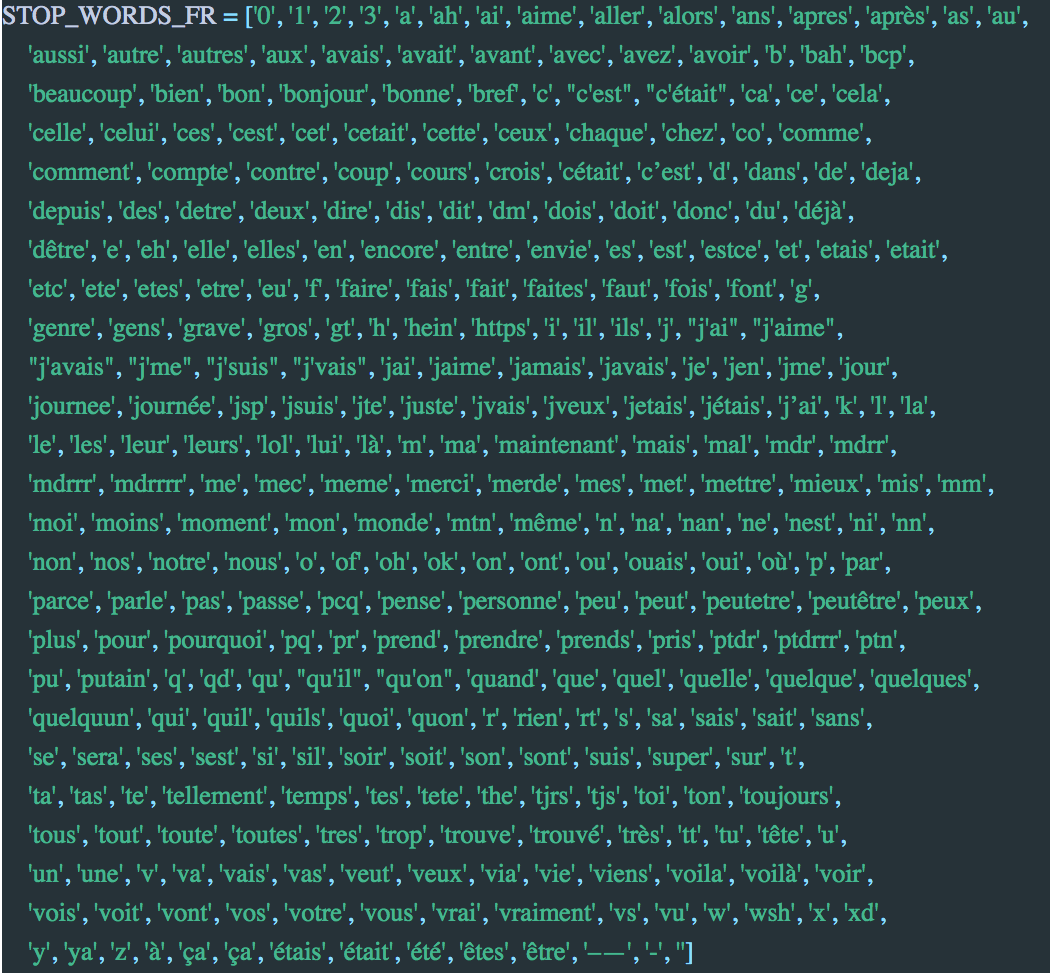
\includegraphics[scale=.7]{figures/stop_words.png}
\end{center}
\vspace{.5cm}	
	\caption{List of stop-words}
	\label{fig:stop_words}
\end{figure}
%%%%%%%%%%%%%%%%%%%%%%%%%%%%%%%%%%%%%%%%%%%%%%%%%%%%%%%%%%%%%%%%%%%%%% 


\clearpage 
\pagebreak


%%%%%%%%%%%%%%%%%%%%%%%%%%%%%%%%%%%%%%%%%
\section{News media content data\label{Sec:OA_Content}}
%%%%%%%%%%%%%%%%%%%%%%%%%%%%%%%%%%%%%%%%%

The content data is from the OTMedia research projet. This projet was subsidized by the \textit{Agence Nationale de la Recherche} (ANR -- National Agency for Research), a French institution tasked with funding scientific research. The INA (\textit{Institut National de l'Audiovisuel} -- National Audiovisual Institute, a repository of all French radio and television audiovisual archives) was the project leader. The OTMedia research projet used the RSS feeds of the media outlets to track every piece of content they produced online. For the media outlets whose RSS feeds were not tracked by INA, we complete the OTMedia data by scrapping the Sitemaps of their website. Finally, we get all the AFP dispatches directly from the AFP.

Our dataset includes the following media outlets:

\begin{multicols}{2}
\textbf{Local daily newspapers:}
	\begin{enumerate}
	\item \textit{L'Ardennais};
	\item  \textit{Aisne Nouvelle};
	\item \textit{Le Berry Republicain};
	\item \textit{La Charente Libre};
	\item \textit{Le Courrier Picard};
	\item \textit{La Depeche Du Midi};
	\item \textit{Est Eclair};
	\item \textit{L'Eveil De La Haute Loire};
	\item \textit{L'Independant Pyrenees Orientales};
	\item \textit{Le Journal De La Haute Marne};
	\item \textit{Le Midi Libre};
	\item \textit{Monaco Matin};
	\item \textit{La Montagne};
	\item \textit{Nice Matin};
	\item \textit{La Nouvelle Republique Des Pyrenees};
	\item \textit{La Nouvelle Republique Du Centre Ouest};
	\item \textit{Ouest France};
	\item \textit{Le Parisien};
	\item \textit{Le Petit Bleu D'Agen};
	\item \textit{La Provence};
	\item \textit{La Republique Des Pyrenees};
	\item \textit{Sud Ouest};
	\item \textit{Le Telegramme};
	\item \textit{L' Union};
	\item \textit{Var Matin};
	\item \textit{La Voix Du Nord};
	\item \textit{Yonne Republicaine}.
	\end{enumerate}
\end{multicols} 	

\begin{multicols}{2}
\textbf{National daily newspapers:}
	\begin{enumerate}
	\item \textit{La Croix};
	\item \textit{Les Echos};
	\item \textit{L'Equipe};
	\item \textit{Le Figaro};
	\item \textit{France Soir};
	\item \textit{La Gazette Des Communes Des Departements Et Des Regions};
	\item \textit{L'Humanite};
	\item \textit{Liberation};
	\item \textit{Le Monde};
	\item \textit{Le Quotidien De L Art};
	\item \textit{La Tribune}.
	\end{enumerate}		
\medskip
\textbf{Free (national daily) newspapers:}
	\begin{enumerate}
	\item \textit{20 Minutes}.
	\end{enumerate}
\medskip
\textbf{Weekly (national \& local) newspapers:}	
	\begin{enumerate}
	\item \textit{10 Sport};
	\item \textit{Agefi};
	\item \textit{Argus};
	\item \textit{Auto Hebdo};
	\item \textit{L'Avenir De Artois};
	\item \textit{Capital};
	\item \textit{Challenges};
	\item \textit{Closer};
	\item \textit{Courrier International};
	\item \textit{Creuse Agricole Et Rurale};
	\item \textit{L'Echo De La Lys};
	\item \textit{Echo Le Valentinois Drome Ardeche};
	\item \textit{Elle};
	\item \textit{Est Agricole Et Viticole};
	\item \textit{L'Express};
	\item \textit{Grazia};
	\item \textit{Les Inrockuptibles};
	\item \textit{Investir};
	\item \textit{Jeune Afrique};
	\item \textit{Le Journal De Millau};
	\item \textit{Le Journal Du Dimanche};
	\item \textit{L'Hebdo Du Vendredi};
	\item \textit{La Manche Libre};
	\item \textit{Marianne};
	\item \textit{Le Monde Diplomatique};
	\item \textit{Le Moniteur Des Travaux Publics Et Du Batiment};
	\item \textit{L'Obs};
	\item \textit{L'Observateur De Beauvais};
	\item \textit{Paris Match};
	\item \textit{Le Paysan Du Haut Rhin};
	\item \textit{Le Point};
	\item \textit{Point De Vue};
	\item \textit{Le Republicain De L'Essonne};
	\item \textit{La Semaine Dans Le Boulonnais};
	\item \textit{Strategies};
	\item \textit{Tele Z};
	\item \textit{L'Usine Nouvelle};
	\item \textit{Version Femina};
	\item \textit{La Volonte Paysanne De L'Aveyron}.
	\end{enumerate}
\medskip	
\textbf{Monthly (national) newspapers:}
	\begin{enumerate}
	\item \textit{Auto Infos};
	\item \textit{Beaux Arts};
	\item \textit{Causeur};
	\item \textit{Connaissance Des Arts};
	\item \textit{Le Courrier De Floride Etats Unis};
	\item \textit{France Amerique Etats Unis};
	\item \textit{Geo};
	\item \textit{GQ Magazine};
	\item \textit{Japon Infos};
	\item \textit{Marie Claire};
	\item \textit{Marie France};
	\item \textit{Mon Viti};
	\item \textit{Premiere};
	\item \textit{Rav};
	\item \textit{La Revue Des Deux Mondes};
	\item \textit{Science Et Vie};
	\item \textit{Sciences Et Avenir};
	\item \textit{Sciences Humaines};
	\item \textit{Tarx};
	\item \textit{Tetu};
	\item \textit{Vogue};
	\item \textit{Zibeline}.
	\end{enumerate}		
\medskip
\textbf{TV:}
	\begin{enumerate}
	\item BFM TV;
	\item Eurosport;
	\item France 24;
	\item LCI;
	\item Public Senat;
	\item TF1;
	\item TV5 Monde.
	\end{enumerate}
\medskip
\textbf{Radio:}
	\begin{enumerate}
	\item Europe 1;
	\item France Bleu (Radio France);
	\item France Culture (Radio France);
	\item France Inter (Radio France);
	\item France Musique (Radio France);
	\item France Info (also TV);
	\item Radio Classique;
	\item RCF;
	\item RFI;
	\item RTL;
	\item Tendance Ouest.
	\end{enumerate}				
\medskip
\textbf{News agencies:} 
	\begin{enumerate}
	\item Agence France Presse.
%	\item Reuters. \textbf{A RAJOUTER}
	\end{enumerate}	
\medskip
\textbf{Pure online media:}
	\begin{enumerate}
	\item 01 Net;
	\item Actu;
	\item Aleteia;
	\item AOC;
	\item Arboriculture Fruitiere;
	\item Basta;
	\item Boursier Com;
	\item Boursorama;
	\item Bref Eco;
	\item Buzzfeed;
	\item C Net;
	\item Cfnews;
	\item Clubic;
	\item Contrepoints;
	\item Les Echos Du Touquet;
	\item Echos Start;
	\item Echosdunet;
	\item Foot Mercato;
	\item Football;
	\item Gamekult;
	\item Gamergen;
	\item Generation Nouvelles Technologies;
	\item Ginjfo;
	\item Goodplanet Info;
	\item Herault Tribune;
	\item Huffington Post;
	\item Influenth;
	\item Informatique News;
	\item L'ADN;
	\item Le Libre Penseur;
	\item Le Media;
	\item Le Tribunal Du Net;
	\item L'Explicite;
	\item L'Incorrect;
	\item L'Internaute;
	\item LVSL;
	\item Maddyness;
	\item Made In Foot;
	\item Made In Perpignan;
	\item Marsactu;
	\item Mashable;
	\item Medialot;
	\item Mediapart;
	\item Meta Media;
	\item Minutenews;
	\item Mon Cultivar Elevage;
	\item Mondafrique;
	\item Monde Informatique;
	\item Les Moutons Enrages;
	\item Myeurop Info;
	\item Newsly;
	\item Numerama;
	\item Numeriques;
	\item Ohmymag;
	\item Olivieranger;
	\item Paris Depeches;
	\item Le Petit Journal;
	\item Pourquoi Docteur;
	\item Pure Medias;
	\item Purepeople;
	\item Resistance Republicaine;
	\item Rue 89 Lyon;
	\item Rue89 Bordeaux;
	\item Rue89 Strasbourg;
	\item Slate;
	\item Sputniknews;
	\item Toulouse 7;
	\item Toute La Culture;
	\item La Tribune De L Art;
	\item Up Magazine;
	\item L'Usine Digitale.
	\end{enumerate}			
\end{multicols}


%%%%%%%%%%%%%%%%%%%%%%%%%%%%%%%%%%%%%%%%%
\paragraph{French-speaking foreign media}

Further, we also gather the content produced online by the following French-speaking foreign media:
\begin{enumerate}
\item \textit{20 Minutes Suisse} (Switzerland);
\item Quotidien Canada (Canada);
\item \textit{Temps Suisse} (Switzerland);
\item Lequotidien (pure online media from Quebec);
\item Africa Intelligence;
\item Express Mu Ile Maurice;
\item Nouvelles Caledoniennes;
\item Nouvelle Tribune Benin;
\item Wort Luxembourg;
\item Infohaiti Net Haiti.
\end{enumerate}


\clearpage 
\pagebreak

%%%%%%%%%%%%%%%%%%%%%%%%%%%%%%%%%%%%%%%%%
%%%%%%%%%%%%%%%%%%%%%%%%%%%%%%%%%%%%%%%%%
\section{Additional tables \label{Sec:AdTables}}
%%%%%%%%%%%%%%%%%%%%%%%%%%%%%%%%%%%%%%%%%
%%%%%%%%%%%%%%%%%%%%%%%%%%%%%%%%%%%%%%%%%

%%%%%%%%%%%%%%%%%%%%%%%%%%%%%%%%%%%%%%%%%%%%%%%%%%%%%%%%%%%%%%%%%%%%%%
\begin{sidewaystable}
\caption{Summary statistics: Tweets -- split sample (July 2018 - September 2018), before filters}
\begin{center}
	{
\def\sym#1{\ifmmode^{#1}\else\(^{#1}\)\fi}
\begin{tabular}{l*{1}{ccccccc}}
\hline\hline
                    &\multicolumn{7}{c}{}                                                                      \\
                    &        Mean&      St.Dev&         P25&      Median&         P75&         Max&         Obs\\
\hline
\textbf{Characteristics of the tweet}&            &            &            &            &            &            &            \\
Length of the tweet (nb of characters)&         101&          52&          60&          97&         140&       1,121& 428,338,133\\
Number of words     &         6.2&         4.0&         3.0&         6.0&         8.0&         269& 428,338,133\\
=1 if tweet contains an URL&        0.13&        0.33&       0.000&       0.000&       0.000&           1& 428,338,133\\
=1 if the tweet is a retweet&        0.63&        0.48&       0.000&       1.000&       1.000&           1& 428,338,133\\
=1 if the tweet is a reply&        0.17&        0.38&       0.000&       0.000&       0.000&           1& 428,338,133\\
=1 if the tweet is a quote&        0.19&        0.39&       0.000&       0.000&       0.000&           1& 428,338,133\\
\textbf{Popularity of the tweet}&            &            &            &            &            &            &            \\
Number of retweets  &         2.2&       110.4&       0.000&       0.000&       0.000&     117,389& 159,932,748\\
Number of replies   &         0.2&         6.5&       0.000&       0.000&       0.000&      47,892& 159,932,748\\
Number of likes     &         3.7&       177.6&       0.000&       0.000&       0.000&     449,881& 159,932,749\\
\hline\hline
\end{tabular}
}

\end{center}
\begin{spacing}{0.5}
	{\fns \textbf{Notes:} The table gives summary statistics. Time period is July 2018 - September 2018. Variables are values for all the tweets included in our dataset before we applied the filters to remove the bots. Variables are described in more details in the text.} 
\end{spacing}
\label{Tab:sum_stat_tweets_split_sample_bflitre}
\end{sidewaystable} 
%%%%%%%%%%%%%%%%%%%%%%%%%%%%%%%%%%%%%%%%%%%%%%%%%%%%%%%%%%%%%%%%%%%%%%


%%%%%%%%%%%%%%%%%%%%%%%%%%%%%%%%%%%%%%%%%%%%%%%%%%%%%%%%%%%%%%%%%%%%%%
\begin{sidewaystable}
\caption{Summary statistics: Twitter users (full sample; last time the user is observed)}
\begin{center}
	{
\def\sym#1{\ifmmode^{#1}\else\(^{#1}\)\fi}
\begin{tabular}{l*{1}{cccccc}}
\hline\hline
                    &\multicolumn{6}{c}{}                                                         \\
                    &        Mean&      St.Dev&         P25&      Median&         P75&         Max\\
\hline
\textbf{User activity}&            &            &            &            &            &            \\
Total number of tweets&      15,174&      40,642&         286&       2,265&      12,762&   6,183,567\\
Nb of tweets btw first \& last time&          99&         445&           4&           9&          38&      61,203\\
Nb of tweets user has liked&       8,520&      23,184&         158&       1,220&       6,655&   2,831,010\\
Nb of users the account is following&         688&        4549&          88&         211&         519&     1672425\\
\textbf{User identity}&            &            &            &            &            &            \\
Date of creation of the account&   2,014.469&       2.742&       2,012&       2,015&       2,017&       2,018\\
=1 if verified account&       0.005&       0.074&           0&           0&           0&           1\\
=1 if user is a journalist&      0.0012&       0.034&           0&           0&           0&           1\\
=1 if user is a media&           0&           0&           0&           0&           0&           1\\
\textbf{User popularity}&            &            &            &            &            &            \\
Nb of followers     &       2,200&      86,685&          32&         147&         515&  58,775,462\\
Nb of public lists  &          20&         578&           0&           1&           6&   1,028,438\\
\hline
Observations        &   4,222,734&            &            &            &            &            \\
\hline\hline
\end{tabular}
}

\end{center}
\begin{spacing}{0.5}
	{\fns \textbf{Notes:} The table gives summary statistics. Time period is July 2018 - July 2019. Variables are values for all the Twitter users included in our dataset the last time we observe them. Variables are described in more details in the text.} 
\end{spacing}
\label{Tab:table_summary_users_all_last}
\end{sidewaystable} 
%%%%%%%%%%%%%%%%%%%%%%%%%%%%%%%%%%%%%%%%%%%%%%%%%%%%%%%%%%%%%%%%%%%%%%


%%%%%%%%%%%%%%%%%%%%%%%%%%%%
%\clearpage 
%\pagebreak
%\begin{table}
%\caption{Summary statistics: Tweets in SMEs and not in SMEs}
%\begin{center}
%{
\def\sym#1{\ifmmode^{#1}\else\(^{#1}\)\fi}
\begin{tabular}{l*{1}{ccc}}
\hline\hline
                    &\multicolumn{3}{c}{ }                          \\
                    &Not in event&    In event&     Diff/se         \\
\hline
\textbf{Characteristics of the tweet}&            &            &                     \\
Length of the tweet (nb of characters)&         134&          73&          61\sym{***}\\
                    &            &            &       (0.0)         \\
Number of words     &           9&           5&           4\sym{***}\\
                    &            &            &       (0.0)         \\
=1 if tweet contains an URL&         0.1&         0.2&      -0.037\sym{***}\\
                    &            &            &     (0.000)         \\
\textbf{Popularity of the tweet}&            &            &                     \\
Number of retweets  &         1.8&         2.5&        -0.7\sym{***}\\
                    &            &            &       (0.0)         \\
Number of replies   &         0.2&         0.2&        -0.0\sym{***}\\
                    &            &            &       (0.0)         \\
Number of likes     &         3.0&         3.8&        -0.8\sym{***}\\
                    &            &            &       (0.0)         \\
\hline
Observations        & 114,698,415&            &                     \\
\hline\hline
\end{tabular}
}

%\end{center} 
%	\begin{spacing}{0.5}
%	{\scriptsize \textbf{Notes:} * p$<$0.10, ** p$<$0.05, *** p$<$0.01. The tables give summary statistics 
%for the characteristics of the tweets in our sample. Time period is July 2018 - September 2018. Column 1 presents the results for the tweets not included in social media events. Column 2 presents the results for the tweets included in social media events. In column 3, we perform a \textit{t}-test on the equality of means.}
%	\end{spacing}
%\label{Tab:sum_stat_tweets_ttest}
%\end{table}
%%%%%%%%%%%%%%%%%%%%%%%%%%%%


%%%%%%%%%%%%%%%%%%%%%%%%%%%%%%%%%%%%%%%%%%%%%%%%%%%%%%%%%%%%%%%%%%%%%%
\begin{table}
\caption{Summary statistics: Joint events -- Depending on news breaker\label{Tab:table_summary_joint_events_ttest}}
\begin{center}
{
\def\sym#1{\ifmmode^{#1}\else\(^{#1}\)\fi}
\begin{tabular}{l*{1}{ccc}}
\hline\hline
                    &\multicolumn{3}{c}{ }                          \\
                    & Media first&Twitter first&     Diff/se         \\
\hline
Length of the event (in hours)&         408&         529&        -120\sym{***}\\
                    &            &            &        (15)         \\
Number of documents in event&       5,678&       4,719&         959         \\
                    &            &            &     (2,171)         \\
\textbf{Twitter coverage}&            &            &                     \\
Nb of tweets in event&       5,623&       4,676&         947         \\
                    &            &            &     (2,170)         \\
Number of different Twitter users&       2,125&       2,957&        -832         \\
                    &            &            &       (467)         \\
Average number of retweets of tweets in events&         2.6&         2.5&         0.0         \\
                    &            &            &       (0.1)         \\
Average number of replys of tweets in events&         0.3&         0.3&        -0.0         \\
                    &            &            &       (0.0)         \\
Average number of favorites of tweets in events&         3.1&         3.7&        -0.6\sym{**} \\
                    &            &            &       (0.2)         \\
\textbf{Media coverage}&            &            &                     \\
Number of news articles in the event&          55&          43&          12\sym{***}\\
                    &            &            &         (3)         \\
Number of different media outlets&          18&          16&           1\sym{**} \\
                    &            &            &         (0)         \\
\hline
Observations        &       5,766&            &                     \\
\hline\hline
\end{tabular}
}

\end{center}
\begin{spacing}{0.5}
{\fns \textbf{Notes:} The table gives summary statistics. Time period is July 2018 - September 2018. The observations are at the event level.  Column 1 presents the events that appear first on media. Column 2 presents the results for the events that appear first on Twitter. In column 3, we perform a \textit{t}-test on the equality of means.}
\end{spacing}
\end{table} 
%%%%%%%%%%%%%%%%%%%%%%%%%%%%%%%%%%%%%%%%%%%%%%%%%%%%%%%%%%%%%%%%%%%%%%


%%%%%%%%%%%%%%%%%%%%%%%%%%%%%%%%%%%%%%%%%%%%%%%%%%%%%%%%%%%%%%%%%%%%%%
\begin{sidewaystable}
\caption{Summary statistics: Twitter users -- Gatekeepers}
\begin{center}
	{
\def\sym#1{\ifmmode^{#1}\else\(^{#1}\)\fi}
\begin{tabular}{l*{1}{cccccc}}
\hline\hline
                    &\multicolumn{6}{c}{}                                                         \\
                    &        Mean&      St.Dev&         P25&      Median&         P75&         Max\\
\hline
\textbf{User activity}&            &            &            &            &            &            \\
Total number of tweets&      65,663&     131,782&       4,700&      21,555&      74,287&   6,183,567\\
Nb of tweets July-September 2018&         112&         580&           4&           9&          43&      46,013\\
Nb tweets user has liked&      20,707&      53,746&         415&       2,913&      15,874&   2,831,010\\
Nb of users the account is following&      11,475&      35,916&         353&       1,053&       7,578&   1,672,425\\
\textbf{User identity}&            &            &            &            &            &            \\
Date of creation of the account&        2012&           3&        2010&        2011&        2014&        2018\\
=1 if verified account&        39.5&        48.9&         0.0&         0.0&       100.0&         100\\
=1 if user is a journalist&        8.45&       27.82&        0.00&        0.00&        0.00&         100\\
=1 if user is a media&       0.757&       8.668&       0.000&       0.000&       0.000&         100\\
\textbf{User popularity}&            &            &            &            &            &            \\
Nb of followers     &     115,010&     727,425&      12,835&      26,462&      57,461&  58,775,462\\
Nb of public lists  &         592&       4,854&          64&         175&         461&   1,028,438\\
\hline
Observations        &      58,521&            &            &            &            &            \\
\hline\hline
\end{tabular}
}

\end{center}
\begin{spacing}{0.5}
	{\fns \textbf{Notes:} The table gives summary statistics. Time period is July 2018 - September 2018. Variables are values for all the ``gatekeepers" included in our dataset the last time we observe them. Gatekeepers are defined as: \textbf{TO BE COMPLETED}} 
\end{spacing}
\label{Tab:table_summary_gatekeepers}
\end{sidewaystable} 
%%%%%%%%%%%%%%%%%%%%%%%%%%%%%%%%%%%%%%%%%%%%%%%%%%%%%%%%%%%%%%%%%%%%%%

%%%%%%%%%%%%%%%%%%%%%%%%%%%%%%%%%%%%%%%%%%%%%%%%%%%%%%%%%%%%%%%%%%%%%%
\clearpage
\pagebreak
\begin{table}
\caption{Naive estimates: Media-level approach, Depending on the number of journalists with a Twitter account}
\begin{center}
	{
\def\sym#1{\ifmmode^{#1}\else\(^{#1}\)\fi}
\begin{tabular}{l*{4}{c}}
\hline\hline
                    &\multicolumn{2}{c}{Low nb of journalists with Twitter}&\multicolumn{2}{c}{High nb of journalists with Twitter}\\\cmidrule(lr){2-3}\cmidrule(lr){4-5}
                    &\multicolumn{1}{c}{(1)}         &\multicolumn{1}{c}{(2)}         &\multicolumn{1}{c}{(3)}         &\multicolumn{1}{c}{(4)}         \\
\hline
Number of articles  &                     &                     &                     &                     \\
Number of tweets    &       0.041\sym{***}&       0.040\sym{***}&       0.044\sym{***}&       0.043\sym{***}\\
                    &     (0.011)         &     (0.010)         &     (0.011)         &     (0.011)         \\
Seed's number of followers&      -0.023         &      -0.025         &      -0.010         &      -0.012         \\
                    &     (0.015)         &     (0.015)         &     (0.011)         &     (0.011)         \\
\hline
Media FEs           &  \checkmark         &  \checkmark         &  \checkmark         &  \checkmark         \\
Month \& DoW FEs    &  \checkmark         &  \checkmark         &  \checkmark         &  \checkmark         \\
Drop media          &                     &  \checkmark         &                     &  \checkmark         \\
Drop multiple       &                     &  \checkmark         &                     &  \checkmark         \\
Observations        &     131,790         &     129,420         &     395,370         &     388,260         \\
Clusters (events)   &       4,393         &       4,314         &       4,393         &       4,314         \\
Marginal Effect     &       0.011         &       0.011         &       0.022         &       0.021         \\
\hline\hline
\end{tabular}
}

\end{center}
\begin{spacing}{0.5}
	{\fns \textbf{Notes:} * p$<$0.10, ** p$<$0.05, *** p$<$0.01. The time period is July 2018 - September 2018. Models are estimated using a negative binomial estimation. Standard errors are clustered at the event level. An observation is a media-news event.  Columns (1) and (3) report the estimates for all the events that appear first on Twitter; in Columns (2) and (4)  we drop the events whose seed is the Twitter account of a media outlet or journalist (``media") as well as the events whose seed broke more than one event during our time period (``multiple"). All specifications include the seed's number of followers as a control, and day-of-the-week, month, and media fixed effects. In Columns (1) and (2) (respectively (3) and (4), we consider the media with a relatively low (respectively relatively high) number of journalists with a Twitter account. The number of tweets is computed \textit{before} the first news article in the event appears and is given in thousands. More details are provided in the text.} 
\end{spacing}
\label{Tab:number_articles_negbinomial_cevent_heterogeneity_nb_journalist_accounts}
\end{table} 
%%%%%%%%%%%%%%%%%%%%%%%%%%%%%%%%%%%%%%%%%%%%%%%%%%%%%%%%%%%%%%%%%%%%%%


%%%%%%%%%%%%%%%%%%%%%%%%%%%%%%%%%%%%%%%%%%%%%%%%%%%%%%%%%%%%%%%%%%%%%%
\clearpage
\pagebreak
\begin{sidewaystable}
\caption{Naive estimates: Media-level approach, Depending on the Social media presence}
\begin{center}
	{
\def\sym#1{\ifmmode^{#1}\else\(^{#1}\)\fi}
\begin{tabular}{l*{6}{c}}
\hline\hline
                    &\multicolumn{3}{c}{Low social media presence}                    &\multicolumn{3}{c}{High social media presence}                   \\\cmidrule(lr){2-4}\cmidrule(lr){5-7}
                    &\multicolumn{1}{c}{(1)}&\multicolumn{1}{c}{(2)}&\multicolumn{1}{c}{(3)}&\multicolumn{1}{c}{(4)}&\multicolumn{1}{c}{(5)}&\multicolumn{1}{c}{(6)}\\
                    &\multicolumn{1}{c}{Number of articles}&\multicolumn{1}{c}{Number of articles}&\multicolumn{1}{c}{Coverage}&\multicolumn{1}{c}{Number of articles}&\multicolumn{1}{c}{Number of articles}&\multicolumn{1}{c}{Coverage}\\
\hline
main                &                     &                     &                     &                     &                     &                     \\
Number of tweets    &       0.033\sym{***}&       0.033\sym{***}&       0.012\sym{***}&       0.055\sym{***}&       0.054\sym{***}&       0.017\sym{***}\\
                    &     (0.008)         &     (0.008)         &     (0.003)         &     (0.013)         &     (0.013)         &     (0.004)         \\
Seed's number of followers&      -0.017         &      -0.017         &      -0.010\sym{**} &      -0.015         &      -0.017         &      -0.009\sym{***}\\
                    &     (0.011)         &     (0.011)         &     (0.004)         &     (0.011)         &     (0.011)         &     (0.004)         \\
\hline
Media FEs           &  \checkmark         &  \checkmark         &  \checkmark         &  \checkmark         &  \checkmark         &  \checkmark         \\
Month \& DoW FEs    &  \checkmark         &  \checkmark         &  \checkmark         &  \checkmark         &  \checkmark         &  \checkmark         \\
Drop media          &                     &  \checkmark         &  \checkmark         &                     &  \checkmark         &  \checkmark         \\
Drop multiple       &                     &  \checkmark         &  \checkmark         &                     &  \checkmark         &  \checkmark         \\
Observations        &     421,728         &     414,144         &     414,144         &     417,335         &     409,830         &     409,830         \\
Clusters (events)   &       4,393         &       4,314         &       4,314         &       4,393         &       4,314         &       4,314         \\
Marginal Effect     &       0.006         &       0.006         &       0.001         &       0.021         &       0.020         &       0.003         \\
\hline\hline
\end{tabular}
}

\end{center}
\begin{spacing}{0.5}
	{\fns \textbf{Notes:} * p$<$0.10, ** p$<$0.05, *** p$<$0.01. The time period is July 2018 - September 2018.  Models are estimated using a negative binomial estimation. Standard errors are clustered at the event level. An observation is a media-news event. We only consider the subset of news events that appear first on Twitter. All specifications include the seed's number of followers as a control, and day-of-the-week, month, and media fixed effects. Columns (1), (3) and (5) report the estimates for all the events that appear first on Twitter; in Columns (2), (4) and (6) we drop the events whose seed is the Twitter account of a media outlet or journalist (``media") as well as the events whose seed broke more than one event during our time period (``multiple"). In Columns (1) and (2) all the media outlets in our sample are included; in Columns (3) and (4) (respectively Columns (5) and (6)) we only consider the media outlets whose social media presence is low (respectively high). High and low social media presence are defined by the share of the media outlet's articles published on social media (above or below the median). The number of tweets is computed \textit{before} the first news article in the event appears and is given in thousands. More details are provided in the text.} 
\end{spacing}
\label{Tab:number_articles_negbinomial_cevent_socialmediapresence}
\end{sidewaystable} 
%%%%%%%%%%%%%%%%%%%%%%%%%%%%%%%%%%%%%%%%%%%%%%%%%%%%%%%%%%%%%%%%%%%%%%




\clearpage 
\pagebreak
%%%%%%%%%%%%%%%%%%%%%%%%%%%%%%%%%%%%%%%%%
%%%%%%%%%%%%%%%%%%%%%%%%%%%%%%%%%%%%%%%%%
%%%%%%%%%%%%%%%%%%%%%%%%%%%%%%%%%%%%%%%%%
\section{Additional figures \label{Sec:AdFigures}}
%%%%%%%%%%%%%%%%%%%%%%%%%%%%%%%%%%%%%%%%%
%%%%%%%%%%%%%%%%%%%%%%%%%%%%%%%%%%%%%%%%%

%%%%%%%%%%%%%%%%%%%%%%%%%%%%%%%%%%%%%%%%%%%%%%%%%%%%%%%%%%%%%%%%%%%%%%
\begin{figure}[ht]
\begin{center}
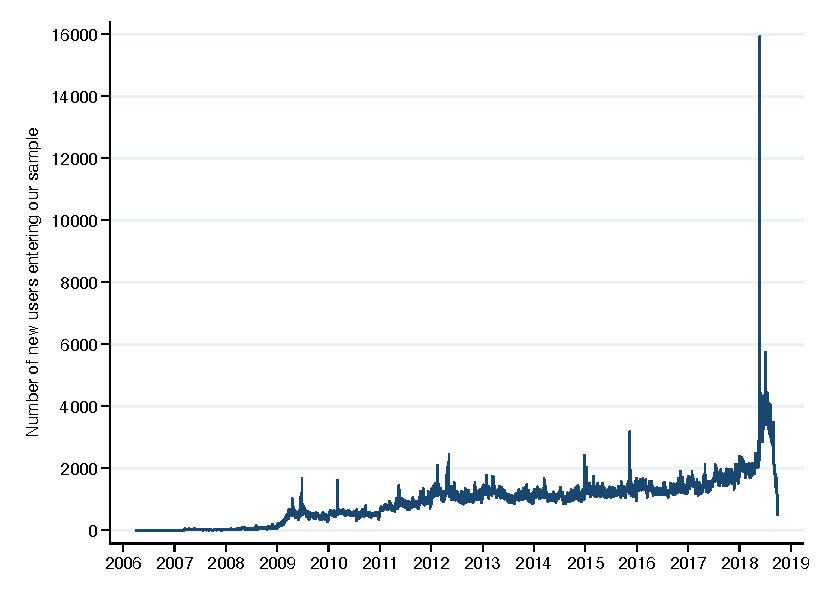
\includegraphics[scale=1]{figures/fig_nb_new_users_daily}
\end{center}
	\begin{spacing}{0.5}
		{\footnotesize \textbf{Notes:} The figure plots the number of users entering our sample depending on the date of their Twitter account creation.}
	\end{spacing}
\vspace{.5cm}	
	\caption{Twitter users: Number of followers depending on the date of their account creation}
	\label{fig:fig_nb_new_users_daily}
\end{figure}
%%%%%%%%%%%%%%%%%%%%%%%%%%%%%%%%%%%%%%%%%%%%%%%%%%%%%%%%%%%%%%%%%%%%%% 


%%%%%%%%%%%%%%%%%%%%%%%%%%%%%%%%%%%%%%%%%%%%%%%%%%%%%%%%%%%%%%%%%%%%%%
\clearpage
\pagebreak
\begin{figure}
\begin{center}
\begin{subfigure}{1\textwidth}
 	    \centering
 	    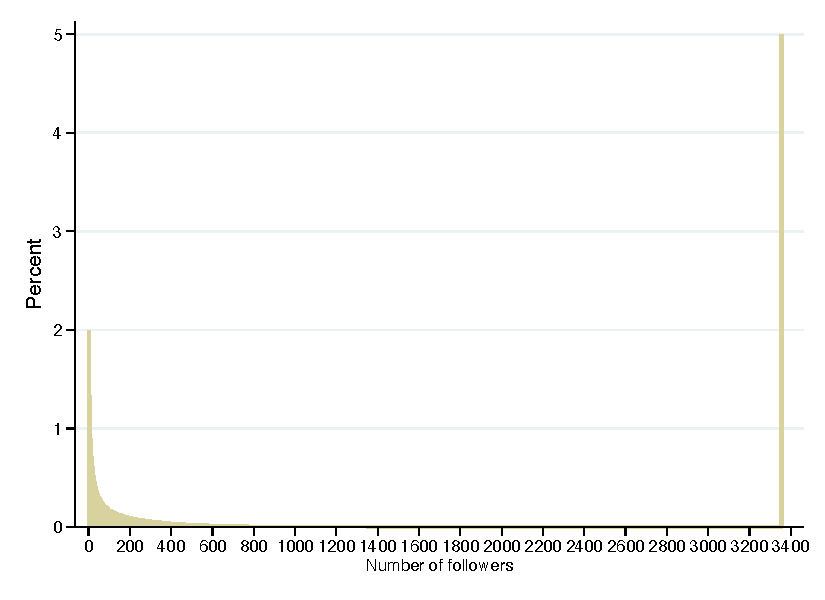
\includegraphics[scale=.9]{figures/distribution_users}
 	    \caption{Distribution of the number of followers}
 	    \label{fig:distribution_users}
\end{subfigure}
\begin{subfigure}{1\textwidth}
 	    \centering
 	    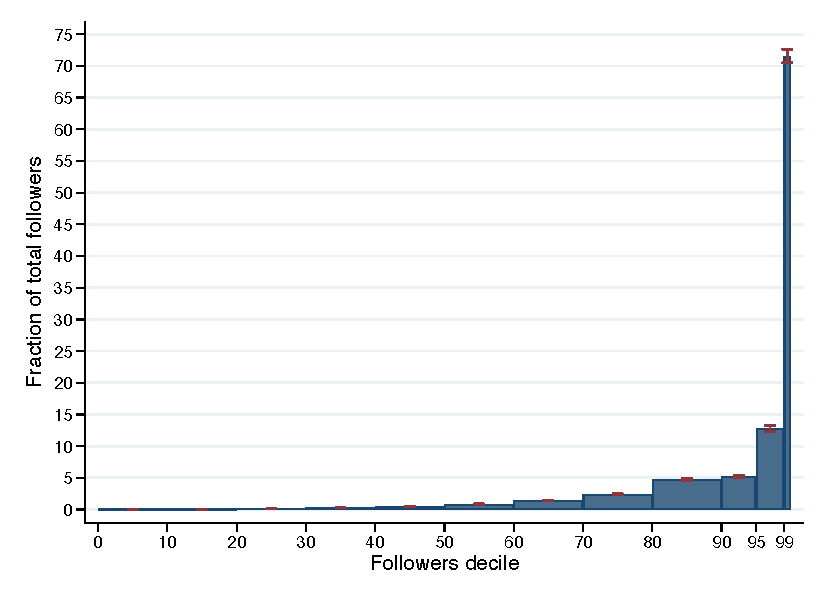
\includegraphics[scale=.9]{figures/cumulative_distribution_followers}
 	    \caption{Cumulative distribution of the number of followers}
 	    \label{fig:cumulative_distribution_followers}
\end{subfigure}
\end{center}
	\begin{spacing}{0.5}
		{\footnotesize \textbf{Notes:} The upper Figure plots the distribution of the number of followers (winsorized at the 95th percentile, i.e. $3,355$ followers) of the Twitter users in our dataset. The bottom Figure plots the cumulative distribution of the number of followers.}
	\end{spacing}
\vspace{.5cm}	
	\caption{Twitter users: Distribution of the number of followers}
	\label{fig:users}
\end{figure}
%%%%%%%%%%%%%%%%%%%%%%%%%%%%%%%%%%%%%%%%%%%%%%%%%%%%%%%%%%%%%%%%%%%%%% 


%%%%%%%%%%%%%%%%%%%%%%%%%%%%%%%%%%%%%%%%%%%%%%%%%%%%%%%%%%%%%%%%%%%%%%
\clearpage
\pagebreak
\begin{figure}
\begin{center}
\begin{subfigure}{1\textwidth}
 	    \centering
 	    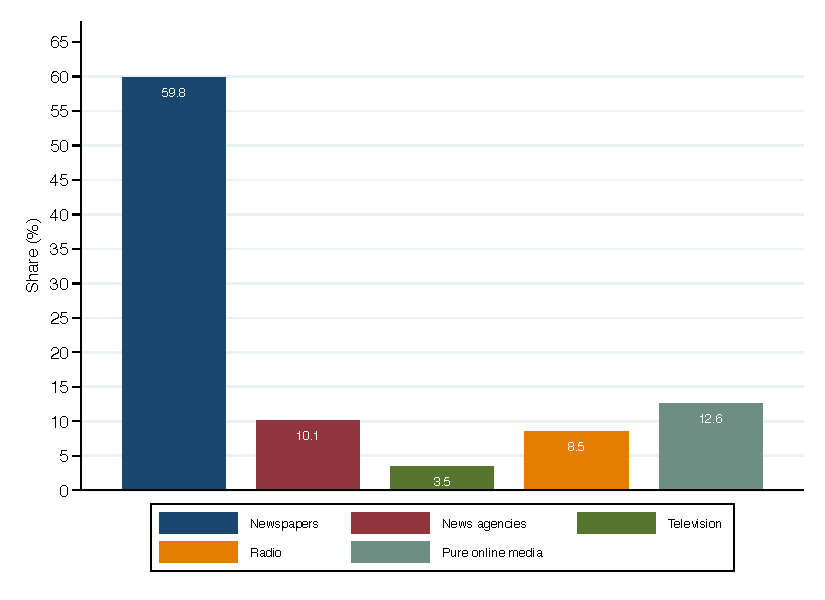
\includegraphics[scale=.6]{figures/share_documents_used_media_category_m}
 	    \caption{All documents}
 	    \label{fig:share_documents_used_media_category_m}
\end{subfigure}
\begin{subfigure}{1\textwidth}
 	    \centering
 	    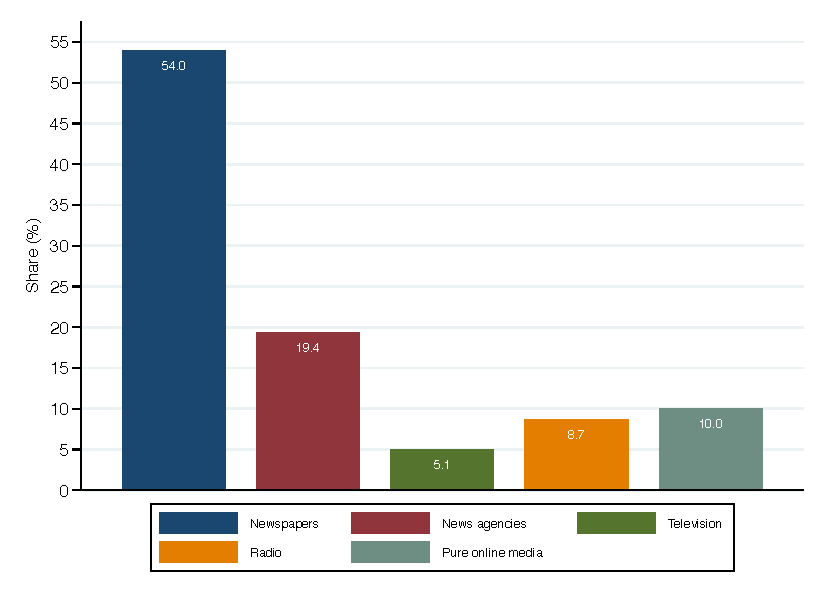
\includegraphics[scale=.6]{figures/share_documents_used_media_category_m_C}
 	    \caption{Documents classified in events}
 	    \label{fig:share_documents_used_media_category_m_C}
\end{subfigure}
\begin{subfigure}{1\textwidth}
 	    \centering
 	    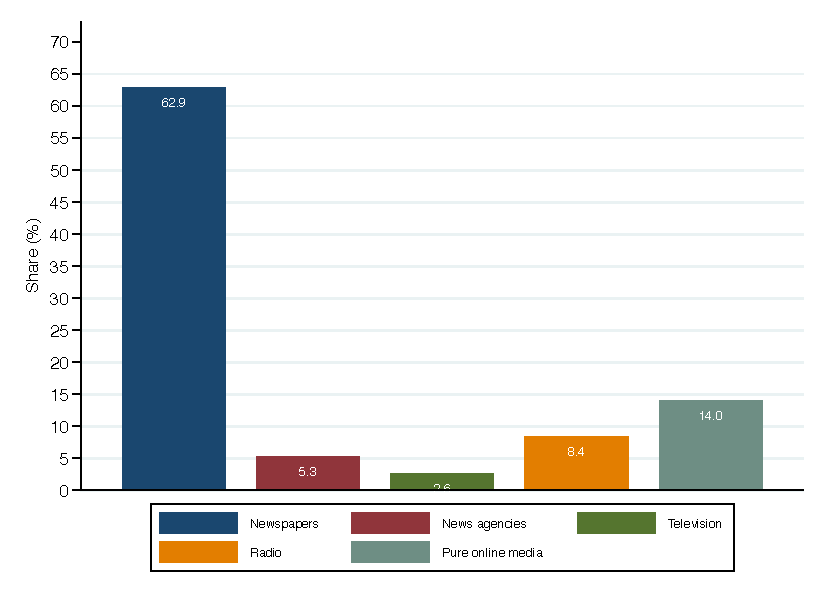
\includegraphics[scale=.6]{figures/share_documents_used_media_category_m_NC}
 	    \caption{Documents not classified in events}
 	    \label{fig:share_documents_used_media_category_m_NC}
\end{subfigure}
\end{center}
	\begin{spacing}{0.5}
		{\footnotesize \textbf{Notes:} The figures plot the share of the documents depending on the offline format of the media outlet. The upper figure \ref{fig:share_documents_used_media_category_m} plots this number for all the documents; the middle figure \ref{fig:share_documents_used_media_category_m_C} for the documents classified in events; and the bottom figure \ref{fig:share_documents_used_media_category_m_NC} for the documents not classified in events. News events are defined in detail in the text, and the list of the media outlets included in each category is given in Section \ref{Sec:OA_Content}.}
	\end{spacing}
\vspace{.5cm}	
	\caption{Share of the documents by offline format}
	\label{fig:share_documents_used_media_category}
\end{figure}



% %%%%%%%%%%%%%%%%%%%%%%%%%%%%%%%%%%%%%%%%%%%%%%%%%%%%%%%%%%%%%%%
% \begin{figure}
% \begin{center}
% \subfloat[][\textbf{English}]{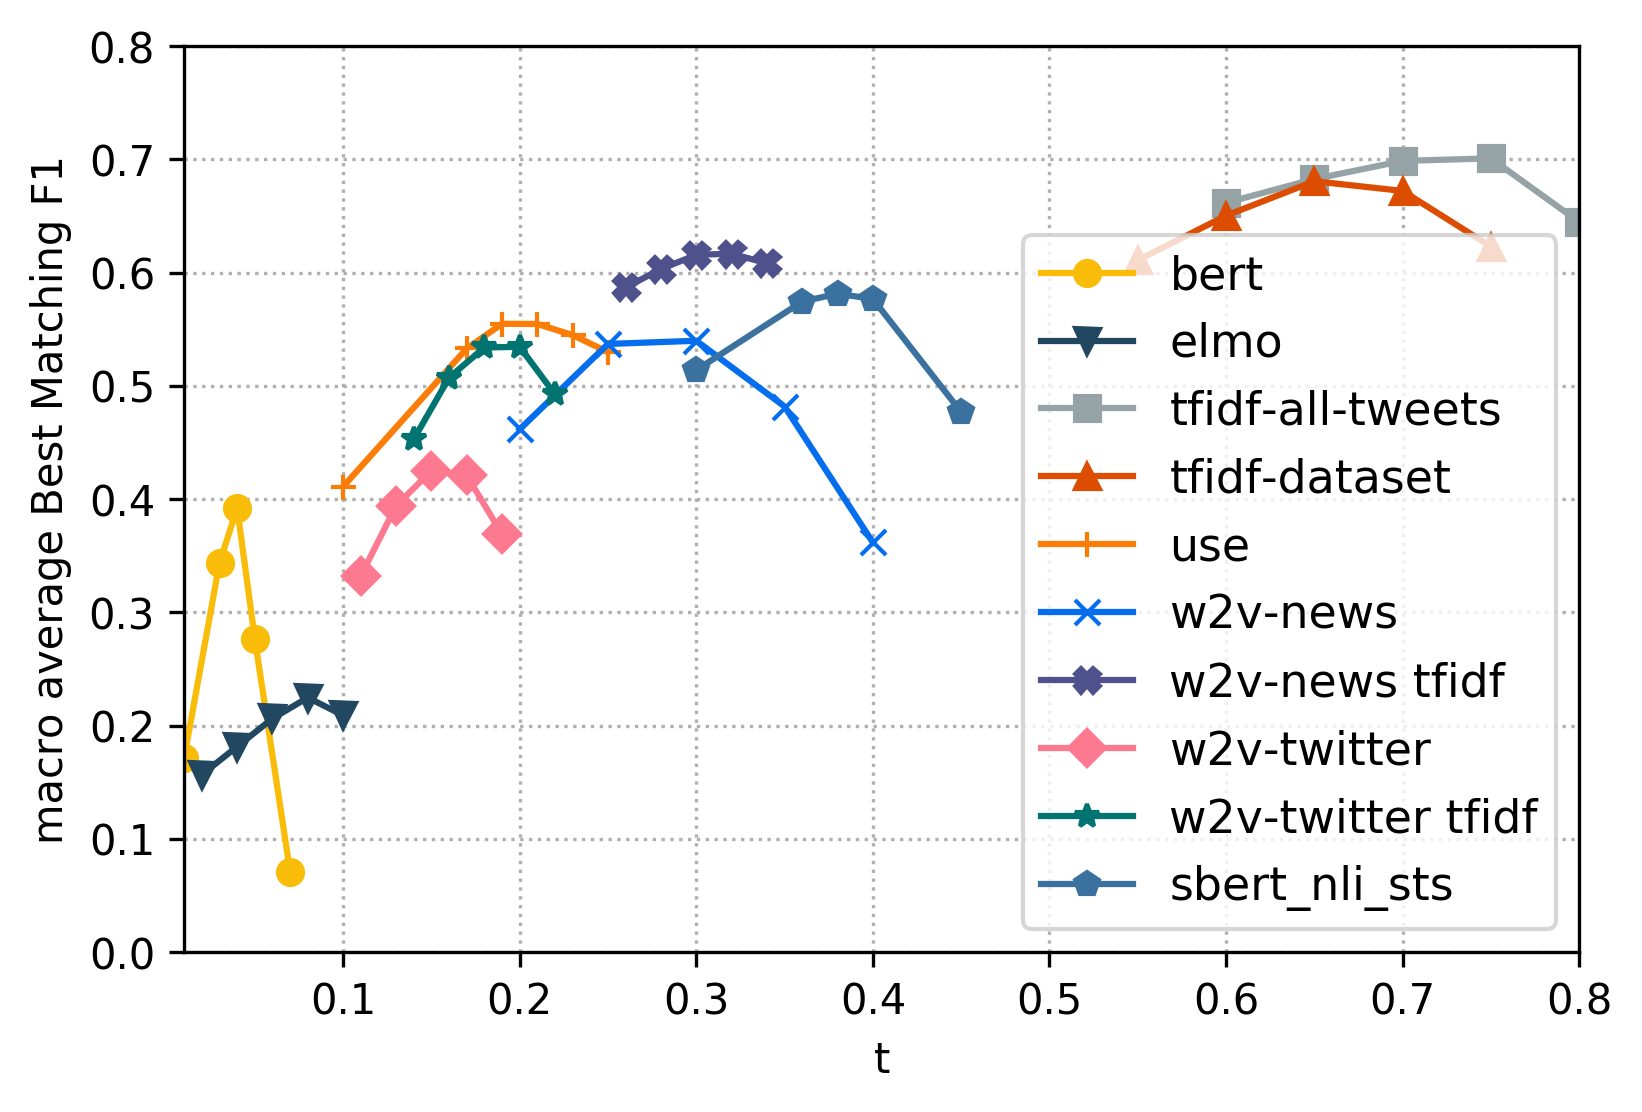
\includegraphics[width=1\linewidth]{figures/Beatrice/graph_en_FSD.png}
% \label{fig: graph_FSD_en}}
% \quad
% \subfloat[][\textbf{French}]{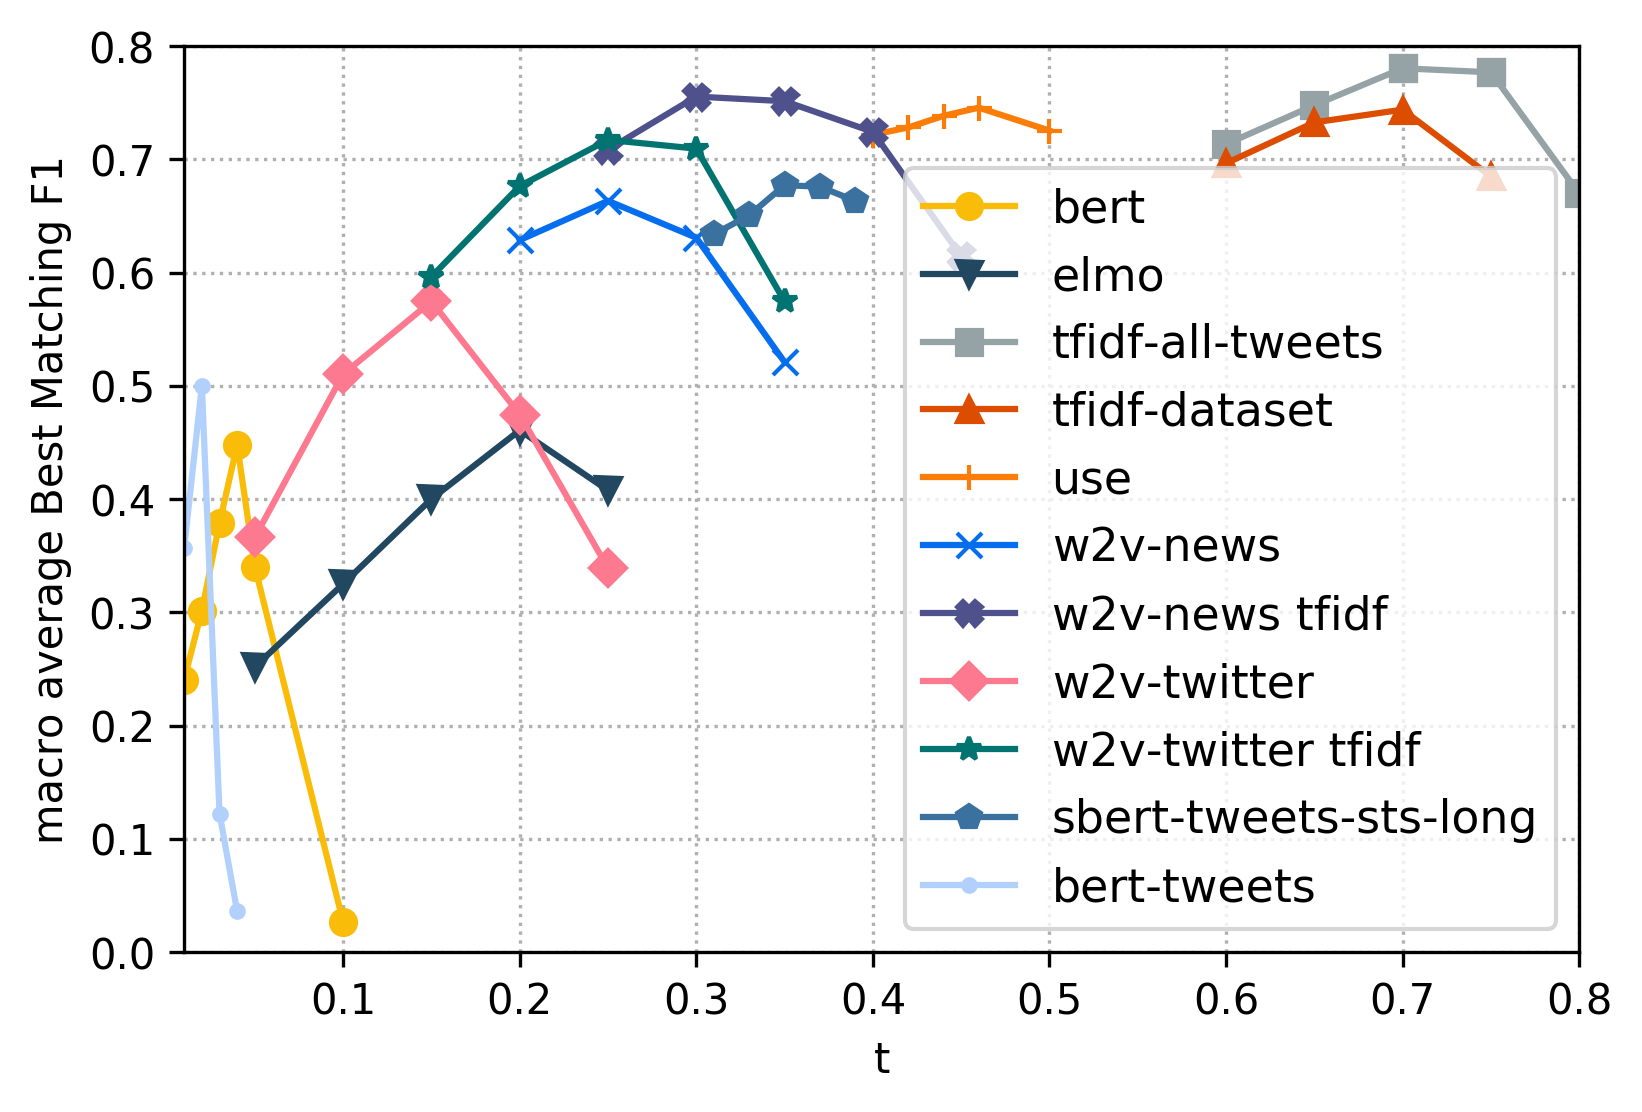
\includegraphics[width=1\linewidth]{figures/Beatrice/graph_fr_FSD.png}
% \label{fig: graph_FSD_fr}}
% \end{center}
% \caption{Best Matching F1 score for FSD clustering depending on the threshold parameter $t$ for each corpus}
% \label{fig: graph_FSD}
% \end{figure}
% %%%%%%%%%%%%%%%%%%%%%%%%%%%%%%%%%%%%%%%%%%%%%%%%%%%%%%%%%%%%%%


%%%%%%%%%%%%%%%%%%%%%%%%%%%%%%%%%%%%%%%%%%%%%%%%%%%%%%%%%%%%%%%%%%%%%%
\clearpage
\pagebreak
\begin{figure}
\begin{center}
\begin{subfigure}{1\textwidth}
 	    \centering
 	    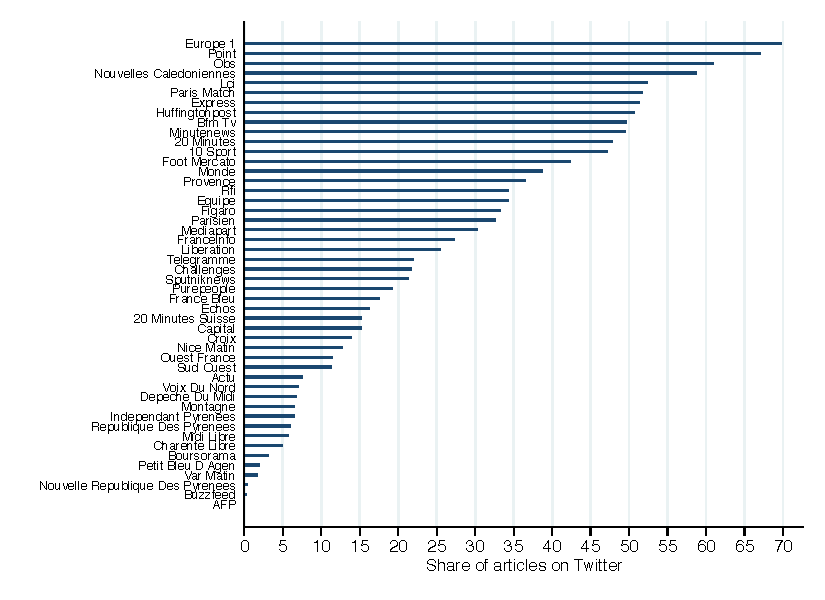
\includegraphics[scale=.6]{figures/fig_mean_Tweeted_fourth_quartile_nb_articles}
 	    \caption{Fourth quartile of the number of articles distribution}
 	    \label{fig:fig_mean_Tweeted_fourth_quartile_nb_articles}
\end{subfigure}
\begin{subfigure}{1\textwidth}
 	    \centering
 	    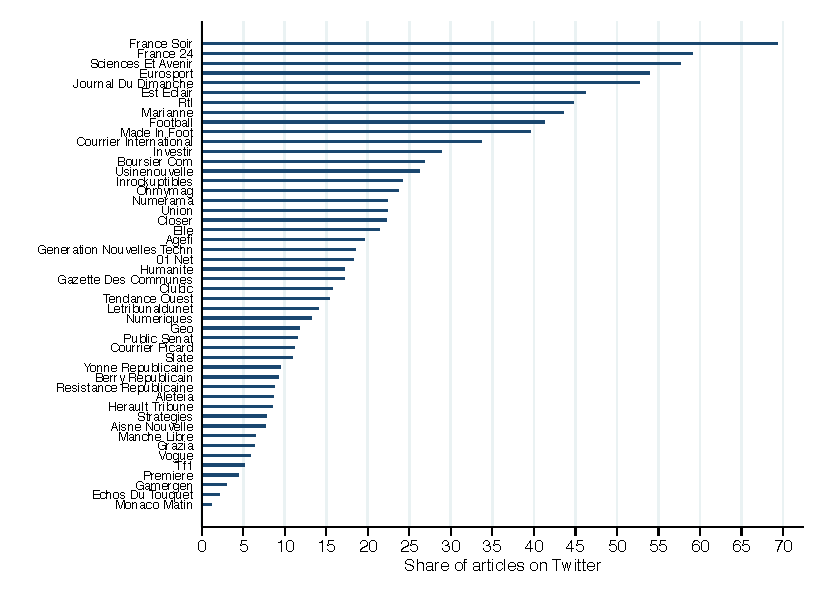
\includegraphics[scale=.6]{figures/fig_mean_Tweeted_third_quartile_nb_articles}
 	    \caption{Third quartile of the number of articles distribution}
 	    \label{fig:fig_mean_Tweeted_third_quartile_nb_articles}
\end{subfigure}
\begin{subfigure}{1\textwidth}
 	    \centering
 	    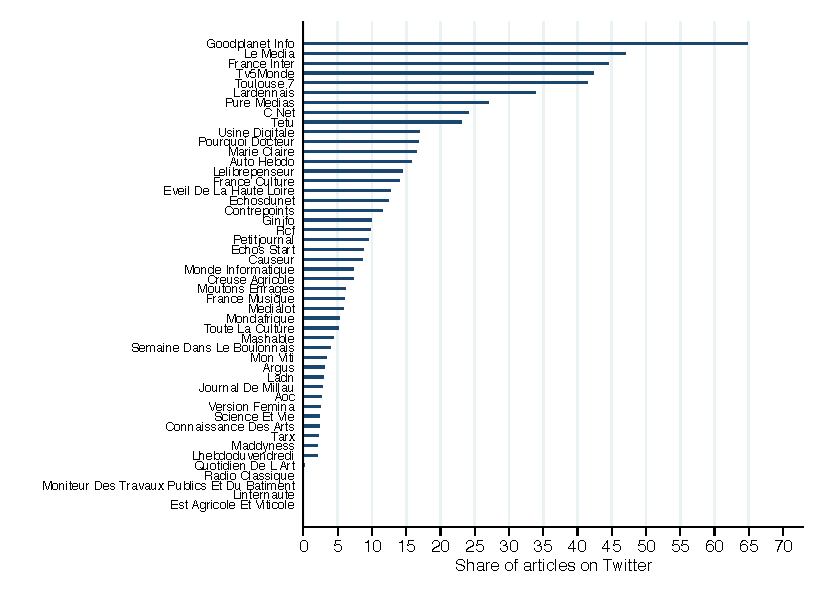
\includegraphics[scale=.6]{figures/fig_mean_Tweeted_second_quartile_nb_articles}
 	    \caption{Second quartile of the number of articles distribution}
 	    \label{fig:fig_mean_Tweeted_second_quartile_nb_articles}
\end{subfigure}
\end{center}
	\begin{spacing}{0.5}
		{\footnotesize \textbf{Notes:} The Figure plot the share of the articles published online that are on Twitter, depending on the media outlet. Media outlets are ranked depending on the number of articles they publish online between July 2018 and September 2018. The upper Figure plots the share for the media outlets that are in the fourth quartile of the number of articles distribution; the middle Figure for the media outlets that are in the third quartile; and the bottom Figure for the media outlets that are in the second quartile.}
	\end{spacing}
\vspace{.5cm}	
	\caption{Share of the articles published online that are on Twitter, depending on the media outlet}
	\label{fig:fig_mean_Tweeted}
\end{figure}


%%%%%%%%%%%%%%%%%%%%%%%%%%%%%%%%%%%%%%%%%%%%%%%%%%%%%%%%%%%%%%%%%%%%%%
\clearpage
\pagebreak
\begin{figure}
\begin{center}
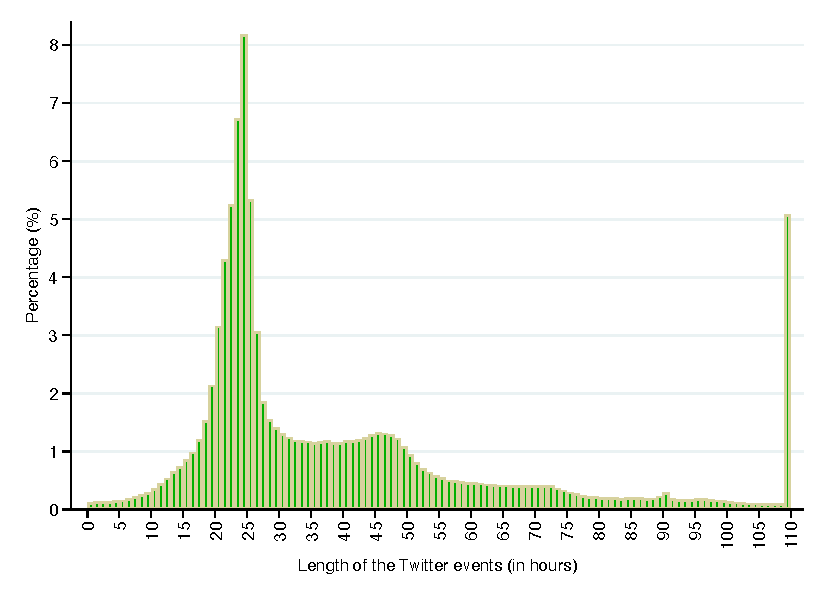
\includegraphics[scale=1]{figures/distribution_length_Tevents}
\end{center}
	\begin{spacing}{0.5}
		{\footnotesize \textbf{Notes:} The figure plots the distribution of the length of the Twitter events (in hours), Winsorized at the 95th percentile (=105 hours). }
	\end{spacing}
\vspace{.5cm}	
	\caption{Twitter events: Distribution of the length of the events}{ Twitter events: Distribution of the length of the events (in hours),
Winsorized at the 95th percentile (=109.8 hours)}
	\label{fig:distribution_length_Tevents}
\end{figure}
%%%%%%%%%%%%%%%%%%%%%%%%%%%%%%%%%%%%%%%%%%%%%%%%%%%%%%%%%%%%%%%%%%%%%% 

%%%%%%%%%%%%%%%%%%%%%%%%%%%%%%%%%%%%%%%%%%%%%%%%%%%%%%%%%%%%%%%%%%%%%%
\clearpage
\pagebreak
\begin{figure}
\begin{center}
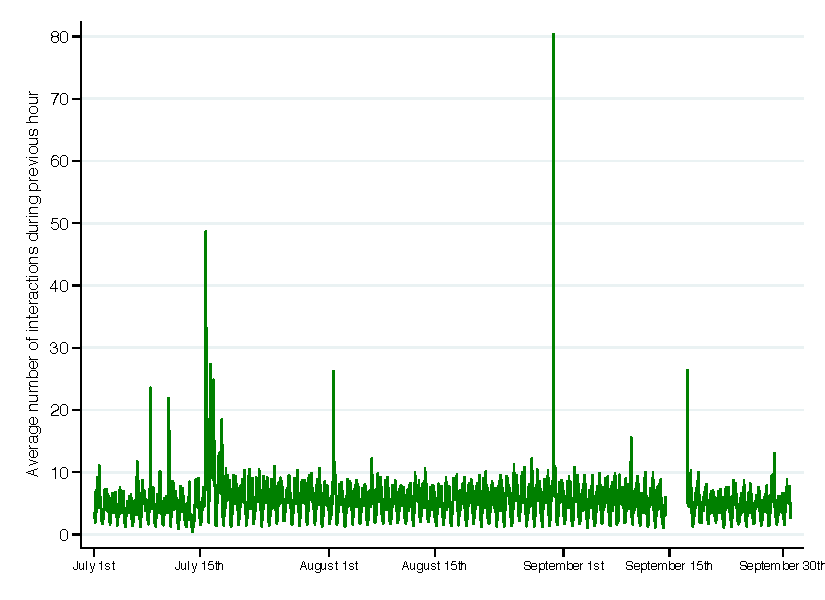
\includegraphics[scale=1]{figures/news_pressure_hour_illustration}
\end{center}
	\begin{spacing}{0.5}
		{\footnotesize \textbf{Notes:} The Figure reports the average number of interactions (retweets/replies/favorites) generated by the tweets published during the previous hour. The average number of interactions is computed at the minute-level.}
	\end{spacing}
\vspace{.5cm}	
	\caption{News pressure: Average number of interactions generated by the tweets published during the previous hour}
	\label{fig:news_pressure_hour_illustration}
\end{figure}
%%%%%%%%%%%%%%%%%%%%%%%%%%%%%%%%%%%%%%%%%%%%%%%%%%%%%%%%%%%%%%%%%%%%%% 

\clearpage 
\pagebreak
%%%%%%%%%%%%%%%%%%%%%%%%%%%%%%%%%%%%%%%%%
%%%%%%%%%%%%%%%%%%%%%%%%%%%%%%%%%%%%%%%%%
\section{Robustness checks \label{Sec:OARobust}}
%%%%%%%%%%%%%%%%%%%%%%%%%%%%%%%%%%%%%%%%%
%%%%%%%%%%%%%%%%%%%%%%%%%%%%%%%%%%%%%%%%%

%%%%%%%%%%%%%%%%%%%%%%%%%%%%%%%%%%%%%%%%%%%%%%%%%%%%%%%%%%%%%%%%%%%%%%
% OK 
\begin{table}[h]
\caption{Naive estimates: Media-level approach, Robustness check: Only media outlets located in France}
\begin{center}
	{
\def\sym#1{\ifmmode^{#1}\else\(^{#1}\)\fi}
\begin{tabular}{l*{4}{c}}
\hline\hline
                    &\multicolumn{2}{c}{Number of articles}     &\multicolumn{2}{c}{=1 if at least one article}\\\cmidrule(lr){2-3}\cmidrule(lr){4-5}
                    &\multicolumn{1}{c}{(1)}         &\multicolumn{1}{c}{(2)}         &\multicolumn{1}{c}{(3)}         &\multicolumn{1}{c}{(4)}         \\
\hline
main                &                     &                     &                     &                     \\
Number of tweets    &       0.048\sym{***}&       0.047\sym{***}&       0.016\sym{***}&       0.016\sym{***}\\
                    &     (0.011)         &     (0.011)         &     (0.003)         &     (0.003)         \\
Seed's number of followers&      -0.016         &      -0.018         &      -0.010\sym{***}&      -0.010\sym{***}\\
                    &     (0.011)         &     (0.011)         &     (0.003)         &     (0.003)         \\
\hline
Media FEs           &  \checkmark         &  \checkmark         &  \checkmark         &  \checkmark         \\
Month \& DoW FEs    &  \checkmark         &  \checkmark         &  \checkmark         &  \checkmark         \\
Drop media          &                     &  \checkmark         &                     &  \checkmark         \\
Drop multiple       &                     &  \checkmark         &                     &  \checkmark         \\
Model               &     Neg bin         &     Neg bin         &      Probit         &      Probit         \\
Observations        &     799,526         &     785,148         &     799,526         &     785,148         \\
Clusters (events)   &       4,393         &       4,314         &       4,393         &       4,314         \\
Marginal Effect     &       0.014         &       0.014         &       0.002         &       0.002         \\
\hline\hline
\end{tabular}
}

\end{center}
\begin{spacing}{0.5}
	{\fns \textbf{Notes:} * p$<$0.10, ** p$<$0.05, *** p$<$0.01. The time period is July 2018 - September 2018.  Models are estimated using a negative binomial estimation. Standard errors are clustered at the event level. An observation is a media-news event. Only the media outlets that are located in France are included. We only consider the subset of news events that appear first on Twitter. All specifications include the seed's number of followers as a control, and day-of-the-week, month, and media fixed effects. Columns (1) and (3) report the estimates for all the events that appear first on Twitter; in Columns (2) and(4) we drop the events whose seed is the Twitter account of a media outlet or journalist (``media") as well as the events whose seed broke more than one event during our time period (``multiple"). In Columns (1) and (2), the dependent variable is the number of articles published by the media in the event. In Columns (3) and (4) the dependent variable is an indicator variable equal to one if the media outlet publishes at least one article in the event and to zero otherwise. The number of tweets is computed \textit{before} the first news article in the event appears and is given in thousands. More details are provided in the text.} 
\end{spacing}
\label{Tab:number_articles_negbinomial_cevent_RFrench}
\end{table} 
%%%%%%%%%%%%%%%%%%%%%%%%%%%%%%%%%%%%%%%%%%%%%%%%%%%%%%%%%%%%%%%%%%%%%%


%%%%%%%%%%%%%%%%%%%%%%%%%%%%%%%%%%%%%%%%%%%%%%%%%%%%%%%%%%%%%%%%%%%%%%
% OK
\clearpage
\pagebreak
\begin{table}
\caption{IV estimates: Media-level approach, Control Function method, Robustness check: Only media outlets located in France}
\begin{center}
	{
\def\sym#1{\ifmmode^{#1}\else\(^{#1}\)\fi}
\begin{tabular}{l*{6}{c}}
\hline\hline
                    &\multicolumn{2}{c}{Reduced form}           &\multicolumn{2}{c}{First stage}            &\multicolumn{2}{c}{Second stage}           \\\cmidrule(lr){2-3}\cmidrule(lr){4-5}\cmidrule(lr){6-7}
                    &\multicolumn{1}{c}{(1)}&\multicolumn{1}{c}{(2)}&\multicolumn{1}{c}{(3)}&\multicolumn{1}{c}{(4)}&\multicolumn{1}{c}{(5)}&\multicolumn{1}{c}{(6)}\\
                    &\multicolumn{1}{c}{Nb articles}&\multicolumn{1}{c}{Nb articles}&\multicolumn{1}{c}{Nb tweets}&\multicolumn{1}{c}{Nb tweets}&\multicolumn{1}{c}{Nb articles}&\multicolumn{1}{c}{Nb articles}\\
\hline
main                &                     &                     &                     &                     &                     &                     \\
\textbf{Instrument} &                     &                     &                     &                     &                     &                     \\
Low*Interactions    &       0.044\sym{**} &       0.045\sym{**} &       0.142\sym{***}&       0.139\sym{***}&                     &                     \\
                    &     (0.020)         &     (0.021)         &     (0.046)         &     (0.047)         &                     &                     \\
\textbf{Controls}   &                     &                     &                     &                     &                     &                     \\
Low                 &       0.135         &       0.128         &       0.169         &       0.164         &       0.126         &       0.120         \\
                    &     (0.082)         &     (0.082)         &     (0.207)         &     (0.208)         &     (0.082)         &     (0.083)         \\
Interactions        &      -0.024\sym{**} &      -0.025\sym{**} &      -0.025         &      -0.026         &      -0.016         &      -0.016         \\
                    &     (0.010)         &     (0.010)         &     (0.030)         &     (0.031)         &     (0.012)         &     (0.012)         \\
Seed’s followers    &      -0.010         &      -0.008         &      -0.037         &      -0.036         &      -0.006         &      -0.004         \\
                    &     (0.014)         &     (0.014)         &     (0.039)         &     (0.040)         &     (0.014)         &     (0.014)         \\
Residuals (1st stage)&                     &                     &                     &                     &       0.046         &       0.048         \\
                    &                     &                     &                     &                     &     (0.109)         &     (0.118)         \\
\textbf{Second stage}&                     &                     &                     &                     &                     &                     \\
Number of tweets    &                     &                     &                     &                     &       0.052\sym{***}&       0.051\sym{***}\\
                    &                     &                     &                     &                     &     (0.012)         &     (0.012)         \\
\hline
Media FEs           &  \checkmark         &  \checkmark         &                     &                     &  \checkmark         &  \checkmark         \\
Month \& DoW FEs    &  \checkmark         &  \checkmark         &  \checkmark         &  \checkmark         &  \checkmark         &  \checkmark         \\
Drop media          &                     &  \checkmark         &                     &  \checkmark         &                     &  \checkmark         \\
Drop multiple       &                     &  \checkmark         &                     &  \checkmark         &                     &  \checkmark         \\
Observations        &     625,170         &     614,068         &     625,170         &     614,068         &     625,170         &     614,068         \\
Clusters (events)   &       3,435         &       3,374         &       3,435         &       3,374         &       3,435         &       3,374         \\
Marginal effect (tweets)&                     &                     &                     &                     &       0.014         &       0.014         \\
\hline\hline
\end{tabular}
}

\end{center}
\begin{spacing}{0.5}
	{\fns \textbf{Notes:} * p$<$0.10, ** p$<$0.05, *** p$<$0.01. The time period is July 2018 - September 2018.  An observation is a media-news event. Only the media outlets that are located in France are included. Standard errors are clustered at the event level. All specifications include the seed's number of followers as a control, and day-of-the-week, month, and media fixed effects. Columns (1) and (2) report the results of the reduced form estimation (the dependent variable is the number of articles), Columns (3) and (4) of the first stage (the dependent variable is the number of tweets), and Columns (5) and (6) of the second stage (the dependent variable is the number of articles). In Columns (2), (4) and (6) we drop the events whose seed is the Twitter account of a media outlet or journalist (``media") as well as the events whose seed broke more than one event during our time period (``multiple"). The number of tweets is computed \textit{before} the first news article in the event appears and is given in thousands. More details are provided in the text.}
\end{spacing}
\label{Tab:regression_media_IV_CF_RFrench}
\end{table} 
%%%%%%%%%%%%%%%%%%%%%%%%%%%%%%%%%%%%%%%%%%%%%%%%%%%%%%%%%%%%%%%%%%%%%%


%%%%%%%%%%%%%%%%%%%%%%%%%%%%%%%%%%%%%%%%%%%%%%%%%%%%%%%%%%%%%%%%%%%%%%
% OK
\clearpage
\pagebreak
\begin{table}
\caption{IV estimates: Media-level approach, IV Poisson GMM, Depending on the offline format, Robustness check: Only media outlets located in France}
\begin{center}
	{
\def\sym#1{\ifmmode^{#1}\else\(^{#1}\)\fi}
\begin{tabular}{l*{6}{c}}
\hline\hline
                    &\multicolumn{1}{c}{Nat. dail.}&\multicolumn{1}{c}{Local dail.}&\multicolumn{1}{c}{Weeklies}&\multicolumn{1}{c}{Pure online}&\multicolumn{1}{c}{TV}&\multicolumn{1}{c}{Radio}\\\cmidrule(lr){2-2}\cmidrule(lr){3-3}\cmidrule(lr){4-4}\cmidrule(lr){5-5}\cmidrule(lr){6-6}\cmidrule(lr){7-7}
                    &\multicolumn{1}{c}{(1)}         &\multicolumn{1}{c}{(2)}         &\multicolumn{1}{c}{(3)}         &\multicolumn{1}{c}{(4)}         &\multicolumn{1}{c}{(5)}         &\multicolumn{1}{c}{(6)}         \\
\hline
Number of articles  &                     &                     &                     &                     &                     &                     \\
Number of tweets    &        0.04\sym{***}&        0.03\sym{**} &        0.05\sym{***}&        0.07\sym{***}&        0.04\sym{***}&       -0.44         \\
                    &      (0.01)         &      (0.01)         &      (0.01)         &      (0.02)         &      (0.01)         &      (6.12)         \\
Low                 &        0.13         &        0.19\sym{**} &        0.14         &       -0.06         &        0.09         &        0.30\sym{**} \\
                    &      (0.10)         &      (0.09)         &      (0.10)         &      (0.12)         &      (0.11)         &      (0.14)         \\
Interactions        &       -0.03\sym{*}  &       -0.02         &       -0.05\sym{**} &       -0.10\sym{**} &       -0.02         &       -0.00         \\
                    &      (0.02)         &      (0.02)         &      (0.02)         &      (0.05)         &      (0.01)         &      (0.01)         \\
Seed’s followers    &        0.00         &        0.00         &        0.01         &        0.00         &        0.00         &        0.01         \\
                    &      (0.02)         &      (0.02)         &      (0.02)         &      (0.02)         &      (0.02)         &      (0.03)         \\
\hline
Media FEs           &  \checkmark         &  \checkmark         &  \checkmark         &  \checkmark         &  \checkmark         &  \checkmark         \\
Month \& DoW FEs    &  \checkmark         &  \checkmark         &  \checkmark         &  \checkmark         &  \checkmark         &  \checkmark         \\
Drop media          &  \checkmark         &  \checkmark         &  \checkmark         &  \checkmark         &  \checkmark         &  \checkmark         \\
Drop multiple       &  \checkmark         &  \checkmark         &  \checkmark         &  \checkmark         &  \checkmark         &  \checkmark         \\
Observations        &      37,114         &      91,098         &     121,464         &     219,310         &      23,618         &      37,114         \\
Clusters (events)   &       3,374         &       3,374         &       3,374         &       3,374         &       3,374         &       3,374         \\
Marginal effect (tweets)&       0.022         &       0.010         &       0.011         &       0.005         &       0.016         &      -0.184         \\
\hline\hline
\end{tabular}
}

\end{center}
\begin{spacing}{0.5}
	{\fns \textbf{Notes:} * p$<$0.10, ** p$<$0.05, *** p$<$0.01. The time period is July 2018 - September 2018. Models are estimated using a a generalized method of moments (GMM) Poisson regression model with endogenous regressors (Stata's ivpoisson command). An observation is a media-news event. Only the media outlets that are located in France are included. We drop the events whose seed is the Twitter account of a media outlet or journalist (``media") as well as the events whose seed broke more than one event during our time period (``multiple"). Standard errors are clustered at the event level. All specifications include the seed's number of followers as a control, and day-of-the-week, month, and media fixed effects.  In Column (1), we only consider the national daily newspapers, in Column (2) the local daily newspapers, in Column (3) the weekly newspapers, in Column (4) the pure online media, in Column (5) the websites of the television stations, and in Column (6) the websites of the radio channels.	The number of tweets is computed \textit{before} the first news article in the event appears and is given in thousands. More details are provided in the text.}
\end{spacing}
\label{Tab:regression_media_IV_Poisson_GMM__RFrench}
\end{table} 
%%%%%%%%%%%%%%%%%%%%%%%%%%%%%%%%%%%%%%%%%%%%%%%%%%%%%%%%%%%%%%%%%%%%%%


%%%%%%%%%%%%%%%%%%%%%%%%%%%%%%%%%%%%%%%%%%%%%%%%%%%%%%%%%%%%%%%%%%%%%%
% OK
\clearpage
\pagebreak
\begin{table}
\caption{Naive estimates: Event-level approach, Robustness check: Controls}
\begin{center}
	{
\def\sym#1{\ifmmode^{#1}\else\(^{#1}\)\fi}
\begin{tabular}{l*{5}{c}}
\hline\hline
                    &\multicolumn{5}{c}{Number of articles}                                                                       \\\cmidrule(lr){2-6}
                    &\multicolumn{1}{c}{(1)}         &\multicolumn{1}{c}{(2)}         &\multicolumn{1}{c}{(3)}         &\multicolumn{1}{c}{(4)}         &\multicolumn{1}{c}{(5)}         \\
\hline
Nb articles         &                     &                     &                     &                     &                     \\
Number of tweets    &       0.057\sym{***}&       0.058\sym{***}&       0.028\sym{***}&       0.028\sym{***}&       0.028\sym{***}\\
                    &     (0.015)         &     (0.015)         &     (0.010)         &     (0.010)         &     (0.011)         \\
Seed's number of followers&      -0.011         &      -0.011         &       0.003         &       0.000         &      -0.001         \\
                    &     (0.011)         &     (0.011)         &     (0.011)         &     (0.013)         &     (0.013)         \\
Reaction time 1st media&                     &                     &       0.199\sym{***}&       0.202\sym{***}&       0.199\sym{***}\\
                    &                     &                     &     (0.018)         &     (0.018)         &     (0.018)         \\
Nb of tweets the seed has liked&                     &                     &                     &      -0.000\sym{*}  &      -0.000\sym{*}  \\
                    &                     &                     &                     &     (0.000)         &     (0.000)         \\
Nb of users the seed's account is following&                     &                     &                     &      -0.000         &      -0.000         \\
                    &                     &                     &                     &     (0.000)         &     (0.000)         \\
Nb of public lists  &                     &                     &                     &       0.000         &       0.000         \\
                    &                     &                     &                     &     (0.000)         &     (0.000)         \\
Seed's total nb of tweets&                     &                     &                     &       0.000         &       0.000         \\
                    &                     &                     &                     &     (0.000)         &     (0.000)         \\
\hline
Month \& DoW FEs    &  \checkmark         &  \checkmark         &  \checkmark         &  \checkmark         &  \checkmark         \\
Drop media          &                     &                     &                     &                     &  \checkmark         \\
Drop multiple       &                     &                     &                     &                     &  \checkmark         \\
Time of the day     &                     &  \checkmark         &  \checkmark         &  \checkmark         &  \checkmark         \\
Observations        &       4,392         &       4,392         &       4,392         &       4,392         &       4,313         \\
Marginal Effect (tweets)&         3.2         &         3.4         &         1.5         &         1.5         &         1.5         \\
\hline\hline
\end{tabular}
}

\end{center}
\begin{spacing}{0.5}
	{\fns \textbf{Notes:} * p$<$0.10, ** p$<$0.05, *** p$<$0.01. The time period is July 2018 - September 2018.  Models are estimated using a negative binomial estimation (robust standard errors are reported between parentheses). An observation is a news event. We only consider the subset of news events that appear first on Twitter. All specifications include the seed's number of followers as a control, and day-of-the-week and month fixed effects. In Columns (2) to (4), we also control for the time of the day of the first tweet (using an indicator variable in hourly format), and in Columns (3) to (5) for the reaction time of the first media (i.e. the time interval between the first tweet in the event and the first news article). In Columns (4) and (5) we also control for the characteristics of the seed of the event; these characteristics are computed the first time we observe the seed in our dataset. Columns (1) to (4) report the estimates for all the events that appear first on Twitter; in Columns (5) we drop the events whose seed is the Twitter account of a media outlet or journalist (``media") as well as the events whose seed broke more than one event during our time period (``multiple"). The number of tweets is computed \textit{before} the first news article in the event appears and is given in thousands. More details are provided in the text.} 
\end{spacing}
\label{Tab:number_articles_negbinomial_event_RControls}
\end{table} 
%%%%%%%%%%%%%%%%%%%%%%%%%%%%%%%%%%%%%%%%%%%%%%%%%%%%%%%%%%%%%%%%%%%%%%


%%%%%%%%%%%%%%%%%%%%%%%%%%%%%%%%%%%%%%%%%%%%%%%%%%%%%%%%%%%%%%%%%%%%%%
% OK
\clearpage
\pagebreak
\begin{table}
\caption{IV estimates: Event-level approach, IV Poisson GMM, Robustness check: Controls}
\begin{center}
	{
\def\sym#1{\ifmmode^{#1}\else\(^{#1}\)\fi}
\begin{tabular}{l*{5}{c}}
\hline\hline
                    &\multicolumn{5}{c}{Number of articles}                                                                       \\\cmidrule(lr){2-6}
                    &\multicolumn{1}{c}{(1)}         &\multicolumn{1}{c}{(2)}         &\multicolumn{1}{c}{(3)}         &\multicolumn{1}{c}{(4)}         &\multicolumn{1}{c}{(5)}         \\
\hline
Nb articles         &                     &                     &                     &                     &                     \\
Number of tweets    &       0.040\sym{***}&       0.033\sym{***}&       0.029\sym{**} &       0.029\sym{**} &       0.030\sym{**} \\
                    &     (0.010)         &     (0.011)         &     (0.012)         &     (0.012)         &     (0.012)         \\
Low                 &       0.171\sym{*}  &       0.201\sym{**} &       0.198\sym{**} &       0.197\sym{**} &       0.190\sym{**} \\
                    &     (0.091)         &     (0.095)         &     (0.095)         &     (0.095)         &     (0.096)         \\
Interactions        &      -0.037\sym{**} &      -0.034\sym{**} &      -0.025         &      -0.029         &      -0.030         \\
                    &     (0.017)         &     (0.017)         &     (0.018)         &     (0.020)         &     (0.020)         \\
Seed's number of followers&       0.003         &       0.003         &       0.013         &       0.013         &       0.014         \\
                    &     (0.017)         &     (0.017)         &     (0.017)         &     (0.019)         &     (0.019)         \\
Reaction time 1st media&                     &                     &       0.206\sym{***}&       0.206\sym{***}&       0.205\sym{***}\\
                    &                     &                     &     (0.034)         &     (0.034)         &     (0.034)         \\
Nb of tweets the seed has liked&                     &                     &                     &      -0.000         &      -0.000         \\
                    &                     &                     &                     &     (0.000)         &     (0.000)         \\
Nb of users the seed's account is following&                     &                     &                     &      -0.000         &      -0.000         \\
                    &                     &                     &                     &     (0.000)         &     (0.000)         \\
Nb of public lists  &                     &                     &                     &       0.000         &       0.000         \\
                    &                     &                     &                     &     (0.000)         &     (0.000)         \\
Seed's total nb of tweets&                     &                     &                     &      -0.000         &      -0.000         \\
                    &                     &                     &                     &     (0.000)         &     (0.000)         \\
\hline
Month \& DoW FEs    &  \checkmark         &  \checkmark         &  \checkmark         &  \checkmark         &  \checkmark         \\
Drop media          &                     &                     &                     &                     &  \checkmark         \\
Drop multiple       &                     &                     &                     &                     &  \checkmark         \\
Observations        &       3,435         &       3,435         &       3,435         &       3,435         &       3,374         \\
Marginal Effect (tweets)&        2.03         &        1.67         &        1.46         &        1.47         &        1.49         \\
\hline\hline
\end{tabular}
}

\end{center}
\begin{spacing}{0.5}
	{\fns \textbf{Notes:} * p$<$0.10, ** p$<$0.05, *** p$<$0.01. The time period is July 2018 - September 2018. Models are estimated using a a generalized method of moments (GMM) Poisson regression model with endogenous regressors (Stata's ivpoisson command). An observation is a news event. Robust standard errors are reported between parentheses. All specifications include the seed's number of followers as a control, and day-of-the-week and month fixed effects. In Columns (2) to (4), we also control for the time of the day of the first tweet (using an indicator variable in hourly format), and in Columns (3) to (5) for the reaction time of the first media (i.e. the time interval between the first tweet in the event and the first news article). In Columns (4) and (5) we also control for the characteristics of the seed of the event; these characteristics are computed the first time we observe the seed in our dataset. Columns (1) to (4) report the estimates for all the events that appear first on Twitter; in Columns (5) we drop the events whose seed is the Twitter account of a media outlet or journalist (``media") as well as the events whose seed broke more than one event during our time period (``multiple").  The number of tweets is computed \textit{before} the first news article in the event appears and is given in thousands. More details are provided in the text.}
\end{spacing}
\label{Tab:regression_event_IV_Poisson_GMM_RControls}
\end{table} 
%%%%%%%%%%%%%%%%%%%%%%%%%%%%%%%%%%%%%%%%%%%%%%%%%%%%%%%%%%%%%%%%%%%%%%


%%%%%%%%%%%%%%%%%%%%%%%%%%%%%%%%%%%%%%%%%%%%%%%%%%%%%%%%%%%%%%%%%%%%%%
% OK
\clearpage
\pagebreak
\begin{table}
\caption{Naive estimates: Event-level approach, Robustness check: Dropping small events}
\begin{center}
	{
\def\sym#1{\ifmmode^{#1}\else\(^{#1}\)\fi}
\begin{tabular}{l*{4}{c}}
\hline\hline
                    &\multicolumn{2}{c}{Number of articles}     &\multicolumn{2}{c}{Number of media}        \\\cmidrule(lr){2-3}\cmidrule(lr){4-5}
                    &\multicolumn{1}{c}{(1)}         &\multicolumn{1}{c}{(2)}         &\multicolumn{1}{c}{(3)}         &\multicolumn{1}{c}{(4)}         \\
\hline
main                &                     &                     &                     &                     \\
Number of tweets    &       0.046\sym{***}&       0.046\sym{***}&       0.018\sym{***}&       0.018\sym{***}\\
                    &     (0.013)         &     (0.013)         &     (0.004)         &     (0.004)         \\
Seed's number of followers&      -0.008         &      -0.009         &      -0.009\sym{**} &      -0.009\sym{**} \\
                    &     (0.011)         &     (0.011)         &     (0.004)         &     (0.004)         \\
\hline
Month \& DoW FEs    &  \checkmark         &  \checkmark         &  \checkmark         &  \checkmark         \\
Drop media          &                     &  \checkmark         &  \checkmark         &  \checkmark         \\
Drop multiple       &                     &  \checkmark         &  \checkmark         &  \checkmark         \\
Observations        &       3,956         &       3,886         &       3,956         &       3,886         \\
Marginal Effect (tweets)&         2.7         &         2.7         &         0.3         &         0.3         \\
\hline\hline
\end{tabular}
}

\end{center}
\begin{spacing}{0.5}
	{\fns \textbf{Notes:} * p$<$0.10, ** p$<$0.05, *** p$<$0.01. The time period is July 2018 - September 2018.  Models are estimated using a negative binomial estimation (robust standard errors are reported between parentheses). An observation is a news event. We only consider the subset of news events that appear first on Twitter, and drop events that in the first decile of the distribution in terms of total number of tweets in the event (``small events"). All specifications include the seed's number of followers as a control, and day-of-the-week and month fixed effects. Columns (1) and (3) report the estimates for all the events that appear first on Twitter; in Columns (2) and (4) we drop the events whose seed is the Twitter account of a media outlet or journalist (``media") as well as the events whose seed broke more than one event during our time period (``multiple"). The number of tweets is computed \textit{before} the first news article in the event appears and is given in thousands. More details are provided in the text} 
\end{spacing}
\label{Tab:number_articles_negbinomial_event_RDropSmallEvents}
\end{table} 
%%%%%%%%%%%%%%%%%%%%%%%%%%%%%%%%%%%%%%%%%%%%%%%%%%%%%%%%%%%%%%%%%%%%%%


%%%%%%%%%%%%%%%%%%%%%%%%%%%%%%%%%%%%%%%%%%%%%%%%%%%%%%%%%%%%%%%%%%%%%%
% OK
\clearpage
\pagebreak
\begin{table}
\caption{IV estimates: Event-level approach, IV Poisson GMM, Robustness check: Dropping small events}
\begin{center}
	{
\def\sym#1{\ifmmode^{#1}\else\(^{#1}\)\fi}
\begin{tabular}{l*{4}{c}}
\hline\hline
                    &\multicolumn{2}{c}{Number of articles}     &\multicolumn{2}{c}{Number of media}        \\\cmidrule(lr){2-3}\cmidrule(lr){4-5}
                    &\multicolumn{1}{c}{(1)}         &\multicolumn{1}{c}{(2)}         &\multicolumn{1}{c}{(3)}         &\multicolumn{1}{c}{(4)}         \\
\hline
main                &                     &                     &                     &                     \\
Number of tweets    &       0.040\sym{***}&       0.041\sym{***}&       0.021\sym{**} &       0.022\sym{**} \\
                    &     (0.010)         &     (0.010)         &     (0.009)         &     (0.009)         \\
Low                 &       0.175\sym{*}  &       0.169\sym{*}  &       0.088\sym{***}&       0.085\sym{***}\\
                    &     (0.094)         &     (0.095)         &     (0.031)         &     (0.031)         \\
Interactions        &      -0.041\sym{**} &      -0.042\sym{**} &       0.001         &       0.000         \\
                    &     (0.017)         &     (0.018)         &     (0.005)         &     (0.005)         \\
Seed’s followers    &       0.006         &       0.007         &      -0.008         &      -0.008         \\
                    &     (0.017)         &     (0.017)         &     (0.005)         &     (0.006)         \\
\hline
Month \& DoW FEs    &  \checkmark         &  \checkmark         &  \checkmark         &  \checkmark         \\
Drop media          &                     &  \checkmark         &                     &  \checkmark         \\
Drop multiple       &                     &  \checkmark         &                     &  \checkmark         \\
Observations        &       3,087         &       3,035         &       3,087         &       3,035         \\
Marginal Effect (tweets)&        2.16         &        2.20         &        0.39         &        0.39         \\
\hline\hline
\end{tabular}
}

\end{center}
\begin{spacing}{0.5}
	{\fns \textbf{Notes:} * p$<$0.10, ** p$<$0.05, *** p$<$0.01. The time period is July 2018 - September 2018. Models are estimated using a a generalized method of moments (GMM) Poisson regression model with endogenous regressors (Stata's ivpoisson command). An observation is a news event.  We only consider the subset of news events that appear first on Twitter, and drop events that in the first decile of the distribution in terms of total number of tweets in the event (``small events"). Robust standard errors are reported between parentheses. All specifications include the seed's number of followers as a control, and day-of-the-week and month fixed effects. In Columns (1) and (2), the dependent variable is the number of articles published in the event. In Columns (3) and (4), the dependent variable in the number of different media outlets covering the event. In Columns (2) and (4) we drop the events whose seed is the Twitter account of a media outlet or journalist (``media") as well as the events whose seed broke more than one event during our time period (``multiple"). The number of tweets is computed \textit{before} the first news article in the event appears and is given in thousands. More details are provided in the text.}
\end{spacing}
\label{Tab:regression_event_IV_Poisson_GMM_RDropSmallEvents}
\end{table} 
%%%%%%%%%%%%%%%%%%%%%%%%%%%%%%%%%%%%%%%%%%%%%%%%%%%%%%%%%%%%%%%%%%%%%%


%%%%%%%%%%%%%%%%%%%%%%%%%%%%%%%%%%%%%%%%%%%%%%%%%%%%%%%%%%%%%%%%%%%%%%
% OK 
\clearpage
\pagebreak
\begin{table}
\caption{IV estimates: Media-level approach, IV Poisson GMM, Depending on the offline format, Robustness check: Only media outlets that published over 90 articles between July and September 2018}
\begin{center}
	{
\def\sym#1{\ifmmode^{#1}\else\(^{#1}\)\fi}
\begin{tabular}{l*{6}{c}}
\hline\hline
                    &\multicolumn{1}{c}{Nat. dail.}&\multicolumn{1}{c}{Local dail.}&\multicolumn{1}{c}{Weeklies}&\multicolumn{1}{c}{Pure online}&\multicolumn{1}{c}{TV}&\multicolumn{1}{c}{Radio}\\\cmidrule(lr){2-2}\cmidrule(lr){3-3}\cmidrule(lr){4-4}\cmidrule(lr){5-5}\cmidrule(lr){6-6}\cmidrule(lr){7-7}
                    &\multicolumn{1}{c}{(1)}         &\multicolumn{1}{c}{(2)}         &\multicolumn{1}{c}{(3)}         &\multicolumn{1}{c}{(4)}         &\multicolumn{1}{c}{(5)}         &\multicolumn{1}{c}{(6)}         \\
\hline
Number of articles  &                     &                     &                     &                     &                     &                     \\
Number of tweets    &        0.04\sym{***}&        0.03\sym{***}&        0.05\sym{***}&        0.07\sym{***}&        0.04\sym{***}&       -0.44         \\
                    &      (0.01)         &      (0.01)         &      (0.01)         &      (0.02)         &      (0.01)         &      (6.12)         \\
Low                 &        0.13         &        0.20\sym{**} &        0.14         &       -0.06         &        0.09         &        0.30\sym{**} \\
                    &      (0.10)         &      (0.09)         &      (0.10)         &      (0.12)         &      (0.11)         &      (0.14)         \\
Interactions        &       -0.03\sym{*}  &       -0.02         &       -0.05\sym{**} &       -0.10\sym{**} &       -0.02         &       -0.00         \\
                    &      (0.02)         &      (0.02)         &      (0.02)         &      (0.05)         &      (0.01)         &      (0.01)         \\
Seed’s followers    &        0.00         &        0.00         &        0.01         &        0.00         &        0.00         &        0.01         \\
                    &      (0.02)         &      (0.02)         &      (0.02)         &      (0.02)         &      (0.02)         &      (0.03)         \\
\hline
Media FEs           &  \checkmark         &  \checkmark         &  \checkmark         &  \checkmark         &  \checkmark         &  \checkmark         \\
Month \& DoW FEs    &  \checkmark         &  \checkmark         &  \checkmark         &  \checkmark         &  \checkmark         &  \checkmark         \\
Drop media          &  \checkmark         &  \checkmark         &  \checkmark         &  \checkmark         &  \checkmark         &  \checkmark         \\
Drop multiple       &  \checkmark         &  \checkmark         &  \checkmark         &  \checkmark         &  \checkmark         &  \checkmark         \\
Observations        &      37,114         &      87,724         &     107,968         &     199,066         &      23,618         &      37,114         \\
Clusters (events)   &       3,374         &       3,374         &       3,374         &       3,374         &       3,374         &       3,374         \\
Marginal effect (tweets)&       0.022         &       0.012         &       0.013         &       0.006         &       0.016         &      -0.184         \\
\hline\hline
\end{tabular}
}

\end{center}
\begin{spacing}{0.5}
	{\fns \textbf{Notes:} * p$<$0.10, ** p$<$0.05, *** p$<$0.01. The time period is July 2018 - September 2018. Models are estimated using a a generalized method of moments (GMM) Poisson regression model with endogenous regressors (Stata's ivpoisson command). An observation is a media-news event. Only the media outlets that published over 90 articles between July and September 2018 are included. We drop the events whose seed is the Twitter account of a media outlet or journalist (``media") as well as the events whose seed broke more than one event during our time period (``multiple"). Standard errors are clustered at the event level. All specifications include the seed's number of followers as a control, and day-of-the-week, month, and media fixed effects.  In Column (1), we only consider the national daily newspapers, in Column (2) the local daily newspapers, in Column (3) the weekly newspapers, in Column (4) the pure online media, in Column (5) the websites of the television stations, and in Column (6) the websites of the radio channels.	The number of tweets is computed \textit{before} the first news article in the event appears and is given in thousands. More details are provided in the text.}
\end{spacing}
\label{Tab:regression_media_IV_Poisson_GMM_R90articles}
\end{table} 
%%%%%%%%%%%%%%%%%%%%%%%%%%%%%%%%%%%%%%%%%%%%%%%%%%%%%%%%%%%%%%%%%%%%%%


% %%%%%%%%%%%%%%%%%%%%%%%%%%%%%%%%%%%%%%%%%
% %%%%%%%%%%%%%%%%%%%%%%%%%%%%%%%%%%%%%%%%% 
\clearpage 
\pagebreak